\documentclass[12pt, letterpaper]{article}
\usepackage[a4paper,left=3cm,right=2cm,top=2.5cm,bottom=2.5cm]{geometry}

\usepackage[utf8]{inputenc}
\usepackage{graphicx}
\graphicspath{ {images/} }
\usepackage{amsmath,bm}
\usepackage{listings}
\usepackage{float}
\usepackage{pdfpages}
\usepackage{siunitx}
\usepackage{subfig}


\title{4TN4 Assignment 2}
\author{Adam Bujak (400113347}
\date{January 31, 2022}

\begin{document}

\maketitle

\section{Theory}


\subsection{Histogram Equalization}

\textbf{Consider the histogram (2, 2, 4, 8, 16, 32, 64, 128) where the number of gray levels is 8 (0-255 intensity levels).
What is the output histogram of histogram equalization?}

To simplify this problem, I will ignore the fact that there are 0-255 intensity levels, and simply take each bin of the histogram as a gray level. The given histogram is shown in Figure \ref{fig:original-histogram}.


\begin{figure}[h]
    \centering
    \includegraphics[width=.8\textwidth]{1-original_histogram.png}
    \caption{Given Histogram}
    \label{fig:original-histogram}
\end{figure}

In Table \ref{tab:histogram-calc} I show the calculated values for the CDF, normalized CDF, and the equalization values.

The equalization values are calculated given the formula below, where $y$ is the normalized CDF value for the gray level, $y'$ is the equalization value, and $L = 8$ (the number of gray levels).

\[ y' =  y \cdot (L-1)\]

\begin{table}[H]
    \centering
    \begin{tabular}{|l|l|l|l|l|}
    \hline
        Gray Level & Frequency & CDF & CDF - Normalized & Equalization  \\ \hline
        0 & 2 & 2 & 0.0078125 & 0  \\
        1 & 2 & 4 & 0.015625 & 0  \\ 
        2 & 4 & 8 & 0.03125 & 0  \\ 
        3 & 8 & 16 & 0.0625 & 0  \\ 
        4 & 16 & 32 & 0.125 & 1  \\ 
        5 & 32 & 64 & 0.25 & 2  \\ 
        6 & 64 & 128 & 0.5 & 4  \\ 
        7 & 128 & 256 & 1 & 7 \\ \hline
    \end{tabular}
    \caption{Calculations}
    \label{tab:histogram-calc}
\end{table}

The calculated equalization values now each represent a new gray level or bin in the new histogram.

By summing the values in the frequency column for each new gray level we can determine the equalized histogram values. For example, for the new gray level of $0$, we see that  $2+2+4+8=16$, and similarly, for the new gray level of $1$, there is only one frequency value which is $16$.

Doing this for each new gray level we get the data in Table \ref{tab:new-histogram}:

\begin{table}[H]
    \centering
    \begin{tabular}{|l|l|}
    \hline
        Gray Level & Frequency  \\ \hline
        0 & 16  \\ 
        1 & 16  \\ 
        2 & 32  \\ 
        3 & 0  \\ 
        4 & 64  \\ 
        5 & 0  \\ 
        6 & 0  \\ 
        7 & 128 \\ \hline
    \end{tabular}
    \caption{New Histogram Values}
    \label{tab:new-histogram}    
\end{table}

In Table \ref{tab:histogram-calc}, we see there are no equalization values with values $3$, $5$, or $6$, therefore, the frequency in those bins of the new histogram are inherently 0.

We can see in Figure \ref{fig:equalized-histogram} that there is a more equalized distribution of gray levels in the new histogram.


\begin{figure}[H]
    \centering
    \includegraphics[width=.8\textwidth]{1-equalized_histogram.png}
    \caption{Equalized Histogram}
    \label{fig:equalized-histogram}
\end{figure}


\subsection{Transfer Function}

\includepdf[pages=3,pagecommand={},width=\textwidth]{transfer-function.pdf}

\subsection{Filtering in Spatial Domain}

Given the following image, we can execute median filtering using the following kernels:
\begin{figure}[H]
    \centering
    $\begin{bmatrix}
    3&5&8&4\\
    9&1&2&9\\
    4&6&7&3\\
    3&8&5&4\\
    \end{bmatrix}$
\end{figure}

\subsubsection{a) Kernel 1}

\begin{figure}[H]
    \centering
    $\begin{bmatrix}
    1&1&1\\
    1&1&1\\
    1&1&1\\
    \end{bmatrix}$
\end{figure}

Given the above kernel and image I will show an example calculation for pixel [1,1] (with value 1). 

To find the pixel value we find the median of the set $3,5,8,9,1,2,4,6,7$. When sorted, the set becomes: $1,2,3,4,5,6,7,8,9$. And we can easily see the median value is $5$.

Doing this for each pixel in the image with 0 padding, we get the following image:

\begin{figure}[H]
    \centering
    $\begin{bmatrix}
    0&2&2&0\\
    3&5&5&3\\
    3&5&5&3\\
    0&4&4&0\\
    \end{bmatrix}$
\end{figure}

\subsubsection{b) Kernel 2}

\begin{figure}[H]
    \centering
    $\begin{bmatrix}
    0&1&0\\
    1&1&1\\
    0&1&0\\
    \end{bmatrix}$
\end{figure}

Given the above kernel and image I will show an example calculation for pixel [1,1] (with value 1). 

To find the pixel value we find the median of the set:

\[[3 \cdot 0],[5 \cdot 1],[8 \cdot 0],[9 \cdot 1],[1 \cdot 1],[2 \cdot 1],[4 \cdot 0],[6 \cdot 1],[7 \cdot 0]\] 

which becomes the set: $0,5,0,9,1,2,0,6,0$.


When sorted, the set becomes: $0,0,0,0,1,2,5,6,9$. And we can easily see the median value is $1$.

Doing this for each pixel in the image with 0 padding, we get the following image:

\begin{figure}[H]
    \centering
    $\begin{bmatrix}
    0&0&0&0\\
    0&1&1&0\\
    0&1&2&0\\
    0&0&0&0\\
    \end{bmatrix}$
\end{figure}

\subsection{Fourier Domain}

\[ a) \xrightarrow{} H. \]
The randomness and noisiness of the bees in the temporal domain are seen by the noisiness and randomness of the frequencies in the Fourier domain.

\[ b) \xrightarrow{} A. \]
A single pair of dots on the y-axis in the Fourier domain is equivalent to horizontal stripes in the temporal domain, and the dot at the origin corresponds to a DC offset.

\[ c) \xrightarrow{} G. \]
As we know, a single pair of diagonal dots centered on the axis of the frequency domain corresponds to a diagonal striped pattern (we know this because it's a rotation of the horizontal stripes). The additional information of the bees and the hexagons of the beehive create the noise we see in the frequency domain and the repeating dots in the higher frequency areas (likely due to the edges of the honeycomb changing quickly). The diagonal grid of dots in the frequency domain corresponds to the hexagonal grid of the beehive.

\[ d) \xrightarrow{} F. \]
There is clearly a low frequency darker area on the fingerprint along approximately \ang{30} line which is evident by looking at the bright spot in the middle of the plot in the frequency domain. Then the random high frequency edges that make up the
ridges of the fingerprint by the outer hazy area in the high frequency region of the frequency plot.

\[ e) \xrightarrow{} B. \]
As we know, a single pair of diagonal dots centered on the axis of the frequency domain corresponds to a diagonal striped pattern (we know this because it's a rotation of the horizontal stripes). So we can clearly tell that these dots correspond to the diagonal stripes of B.

\[ f) \xrightarrow{} E. \]
As we know from the analysis of the checkered pattern of C, a checkered pattern is represented by a pattern like we see in (g). The pattern seen in (f) is similar to that of (g) except with some noise. This indicates that the temporal representation of (f) will be similar to a checkered pattern. The wall is very similar to a checkered pattern, and the noise is just due to the other changes in the picture since it isn't a perfect checkered pattern. We also see a strong vertical line in the frequency domain which is due to the horizontal lines present in the temporal domain at various frequencies.

\[ g) \xrightarrow{} D. \]
We can picture a checkered pattern simply as a combination of a few horizontal and vertical lines at various different frequencies. This is captured perfectly by (g). 
\[ h) \xrightarrow{} D. \]
We can imagine making a circle in the temporal domain by rotating a line \ang{360}. This would cause a circle to be made in the frequency domain as well from what we know about vertical and horizontal lines. Therefore, the frequency domain plot of D. must have a circle in it and (h) is the only one that does.


\section{Implementation}

\subsection{Background Removal}

By getting the median of a every frame of a video with a static background, the moving objects will be removed. If we subtract the remaining image from each frame of the video, only the moving objects will remain.


Figure \ref{fig:background} shows the background of the video extracted using the median technique described above.


\begin{figure}[H]
    \centering
    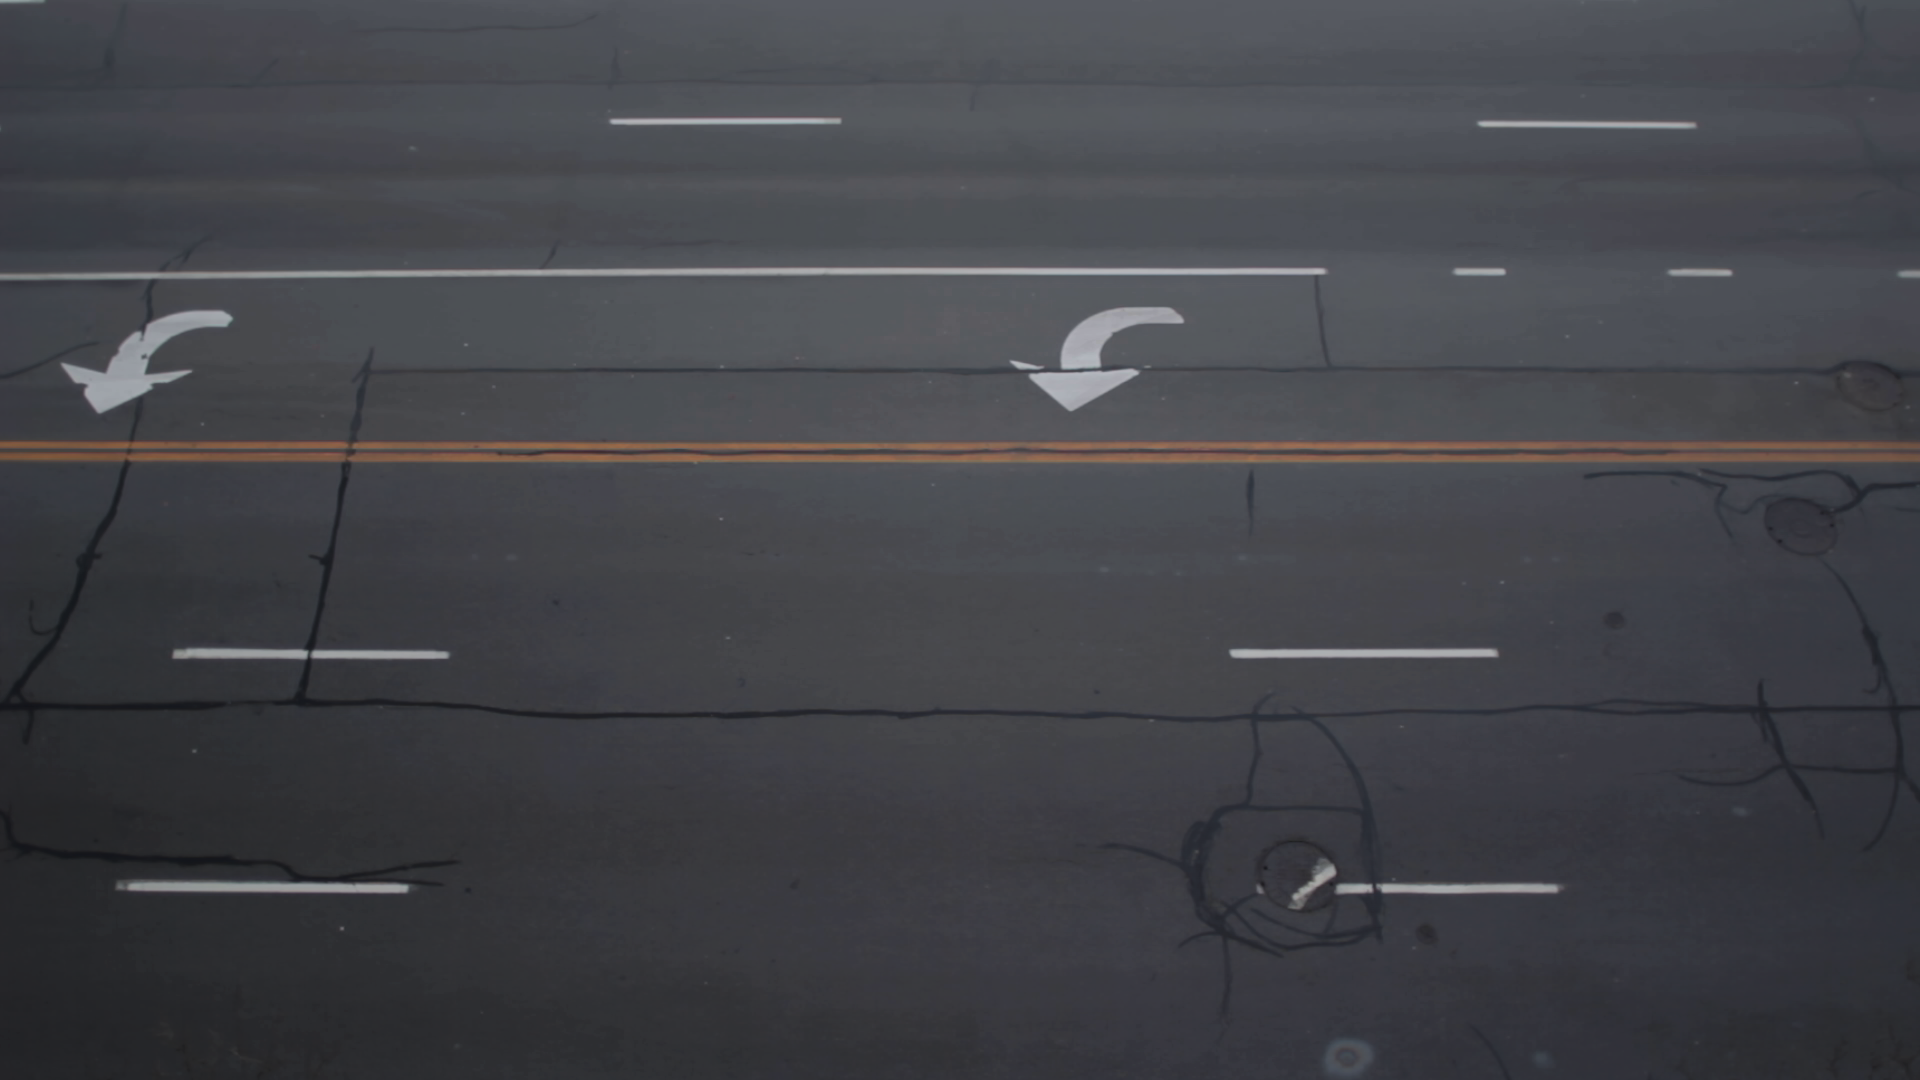
\includegraphics[width=.8\textwidth]{back.png}
    \caption{Static Background of Video}
    \label{fig:background}
\end{figure}

\begin{figure}[H]
    \centering
    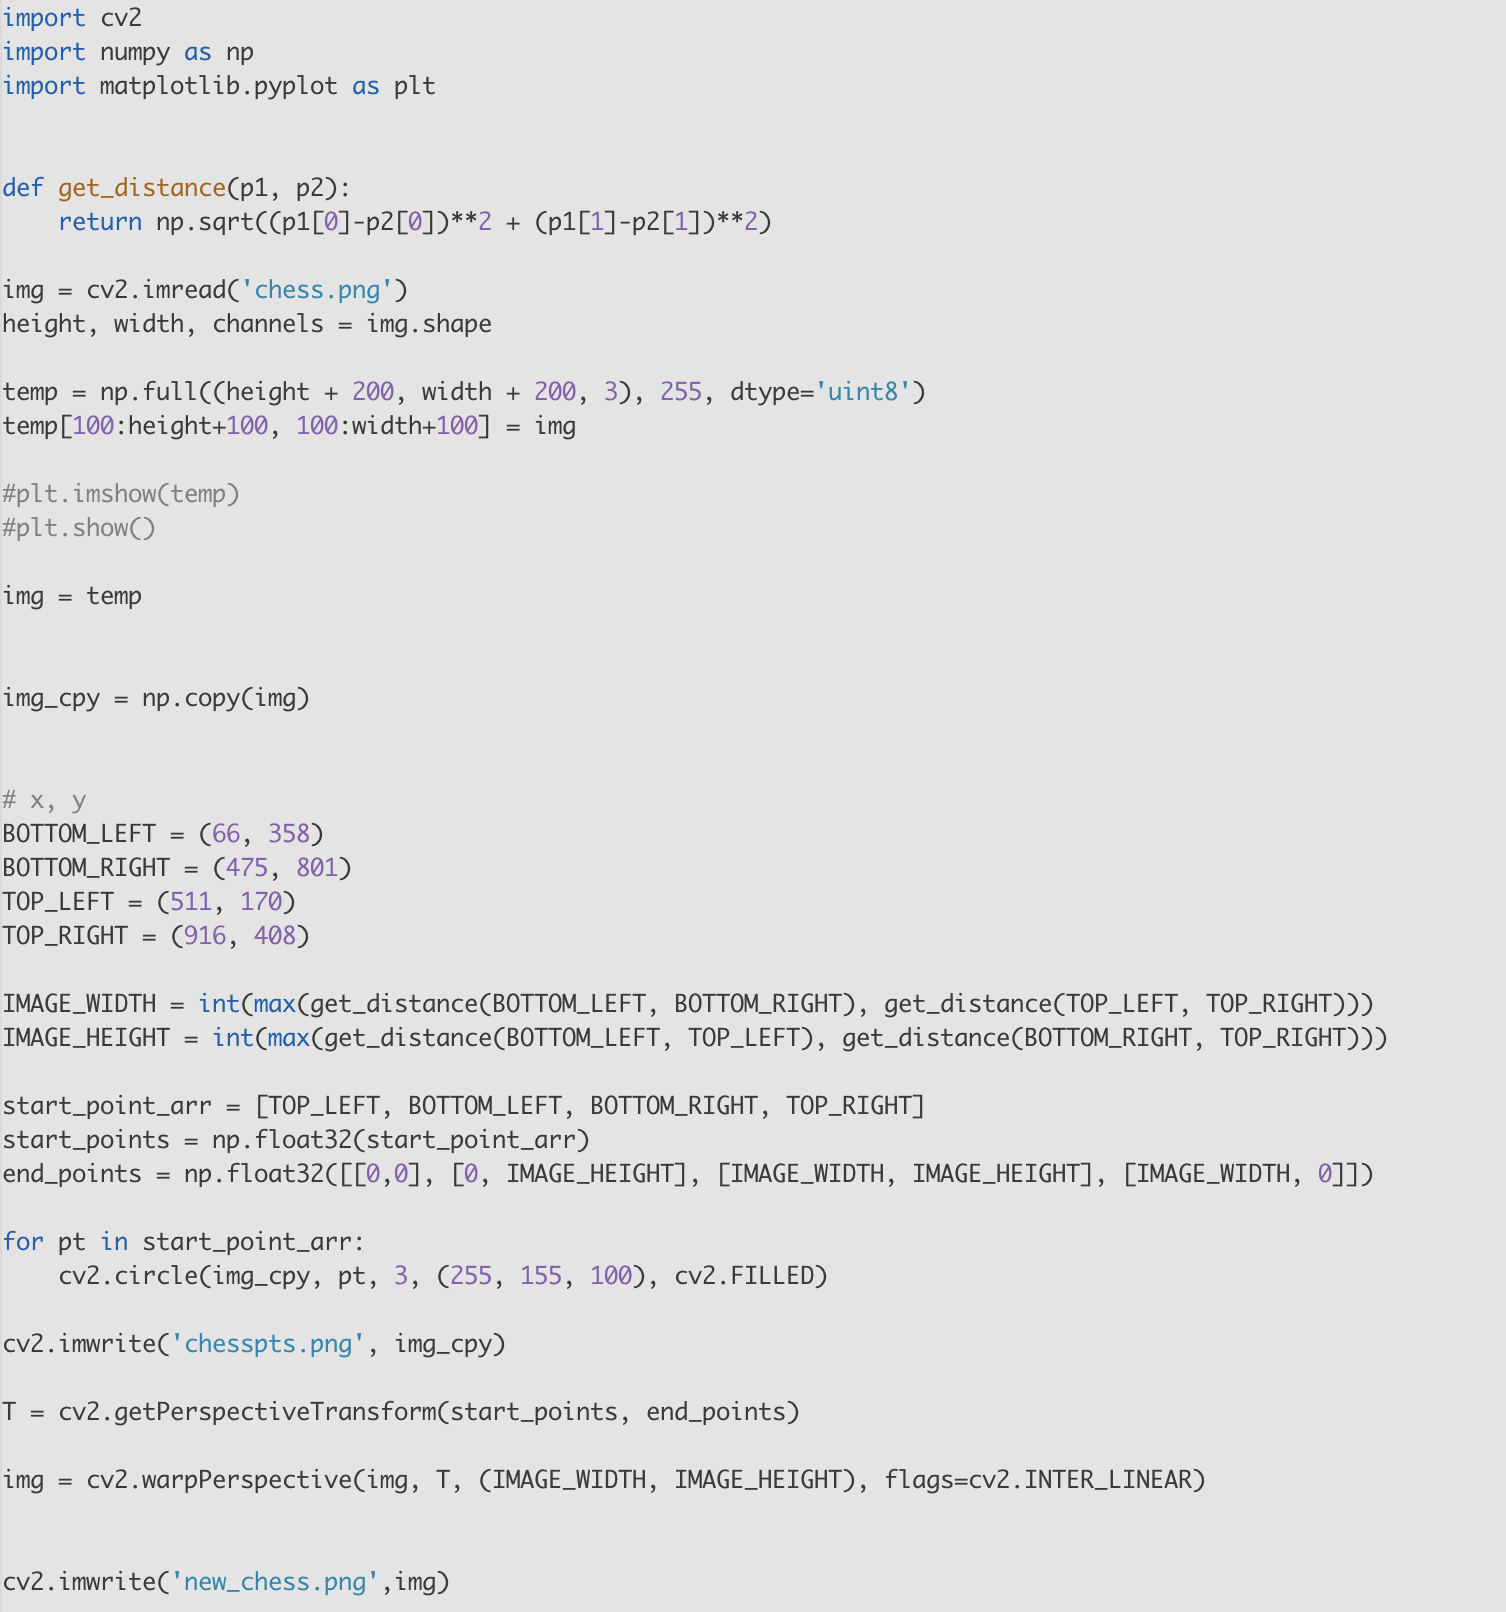
\includegraphics[width=\textwidth]{q1.png}
    \caption{Code for question 1}
    \label{fig:q1}
\end{figure}

\subsection{Image Manipulation in FFT Domain}

From the figures of the soccer players below, we see that the content of the image is mainly contained in the phase of the image. Since we can still clearly see Ronaldo and the other players from that image, and none of Messi in Figure 5, we know that the phase information contains the meaning of the image. The magnitude in the frequency domain contains information about how bright the image should be at every point in the image.

\subsubsection{Phase and Magnitude information}
\begin{figure}[H]
    \centering
    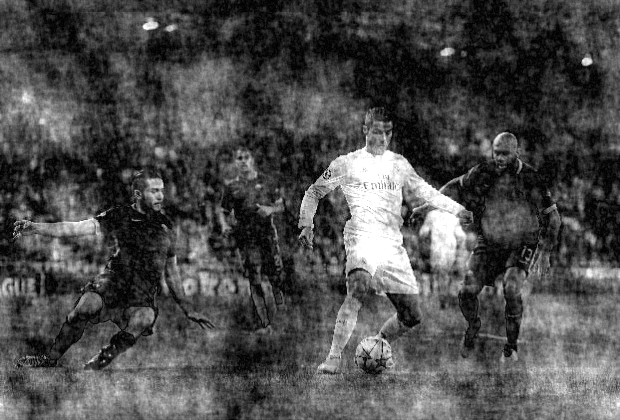
\includegraphics[width=\textwidth]{messi_mag_ronaldo_phase.png}
    \caption{Fourier magnitude of Messi combined with phase of Ronaldo}
\end{figure}

\begin{figure}[H]
    \centering
    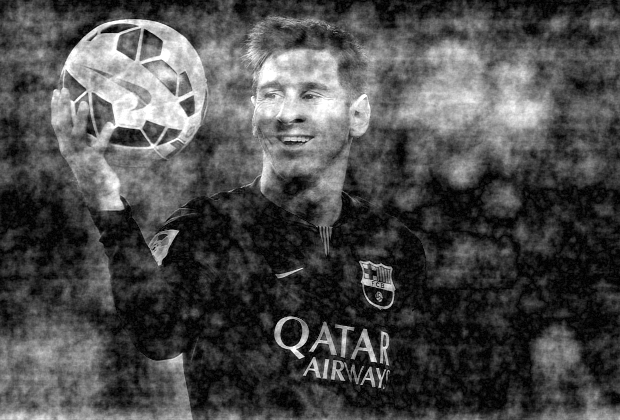
\includegraphics[width=\textwidth]{ronaldo_mag_messi_phase.png}
    \caption{Fourier magnitude of Ronaldo combined with phase of Messi}
\end{figure}

\begin{figure}[H]
    \centering
    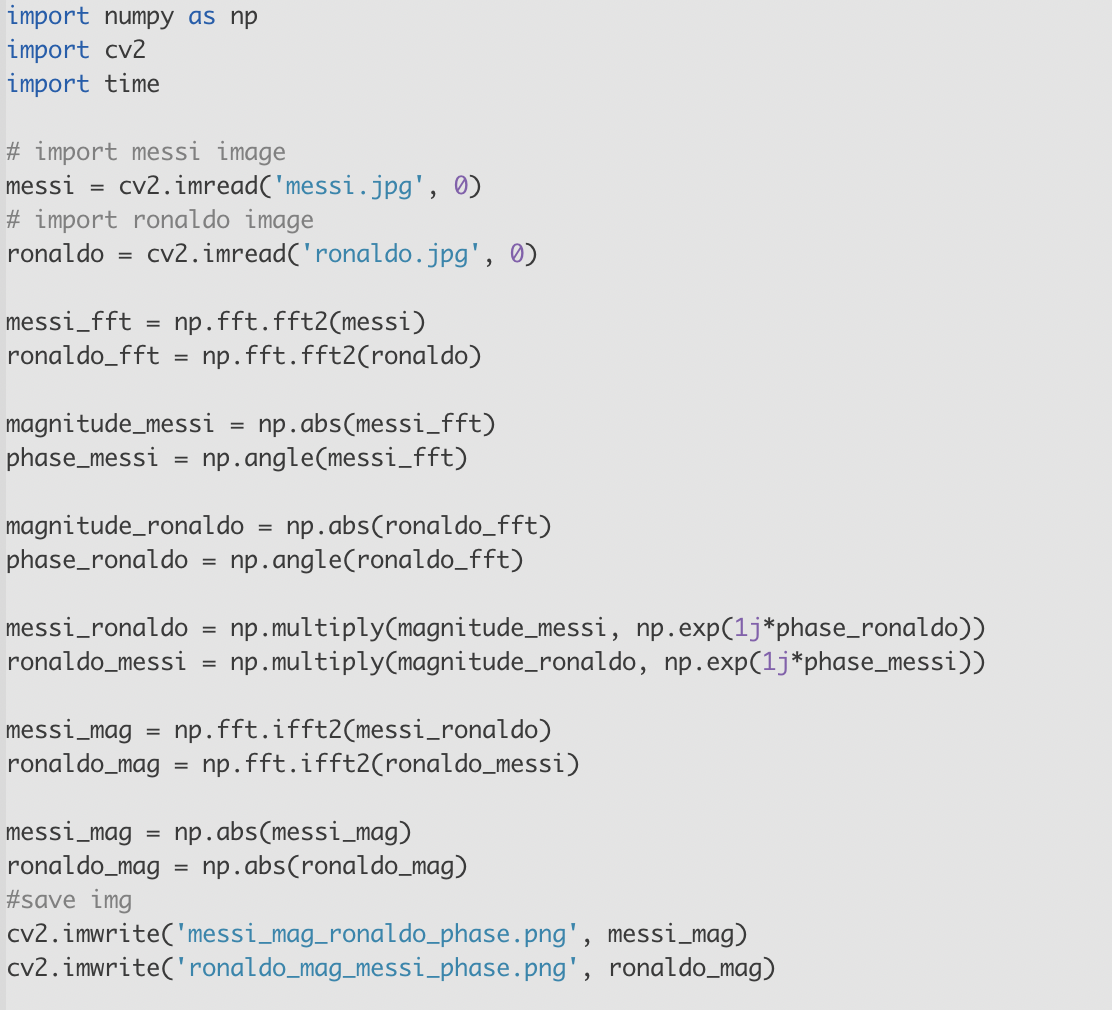
\includegraphics[width=\textwidth]{q2a.png}
    \caption{Phase and Magnitude Separation Code}
\end{figure}

Humans are better at processing low frequency visual information from farther away and high frequency visual information from closer range. When we combine the low-pass filtered image of Messi, with the high-pass filtered image of Ronaldo, in Figure 8 we see Ronaldo more easily, and in Figure 9 we see Messi more easily.
\subsubsection{Fourier Domain Filtering}
\begin{figure}[H]
    \centering
    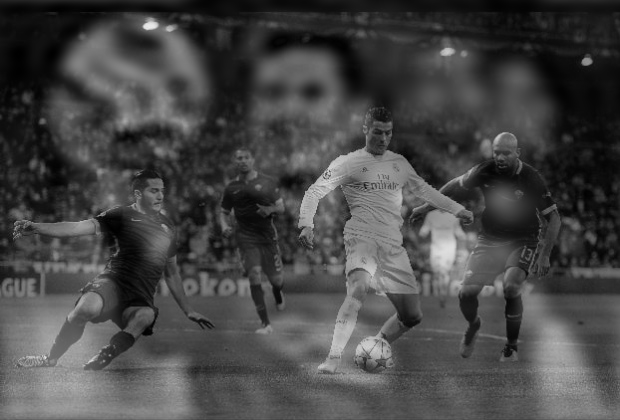
\includegraphics[width=\textwidth]{messi_circle.png}
    \caption{Hybrid Image Close Up}
\end{figure}

\begin{figure}[H]
    \centering
    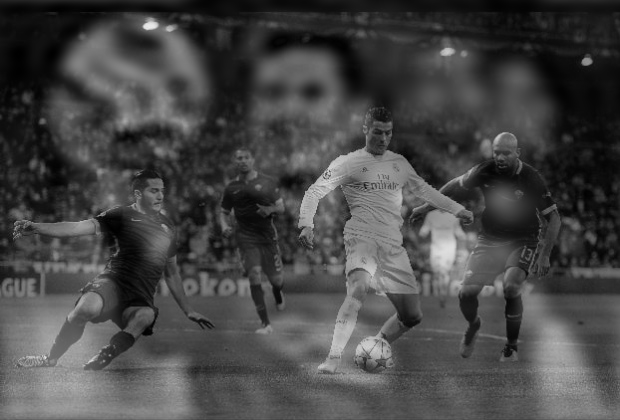
\includegraphics[width=.25\textwidth]{messi_circle.png}
    \caption{Hybrid Image Zoomed Out}
\end{figure}

\begin{figure}[H]
    \centering
    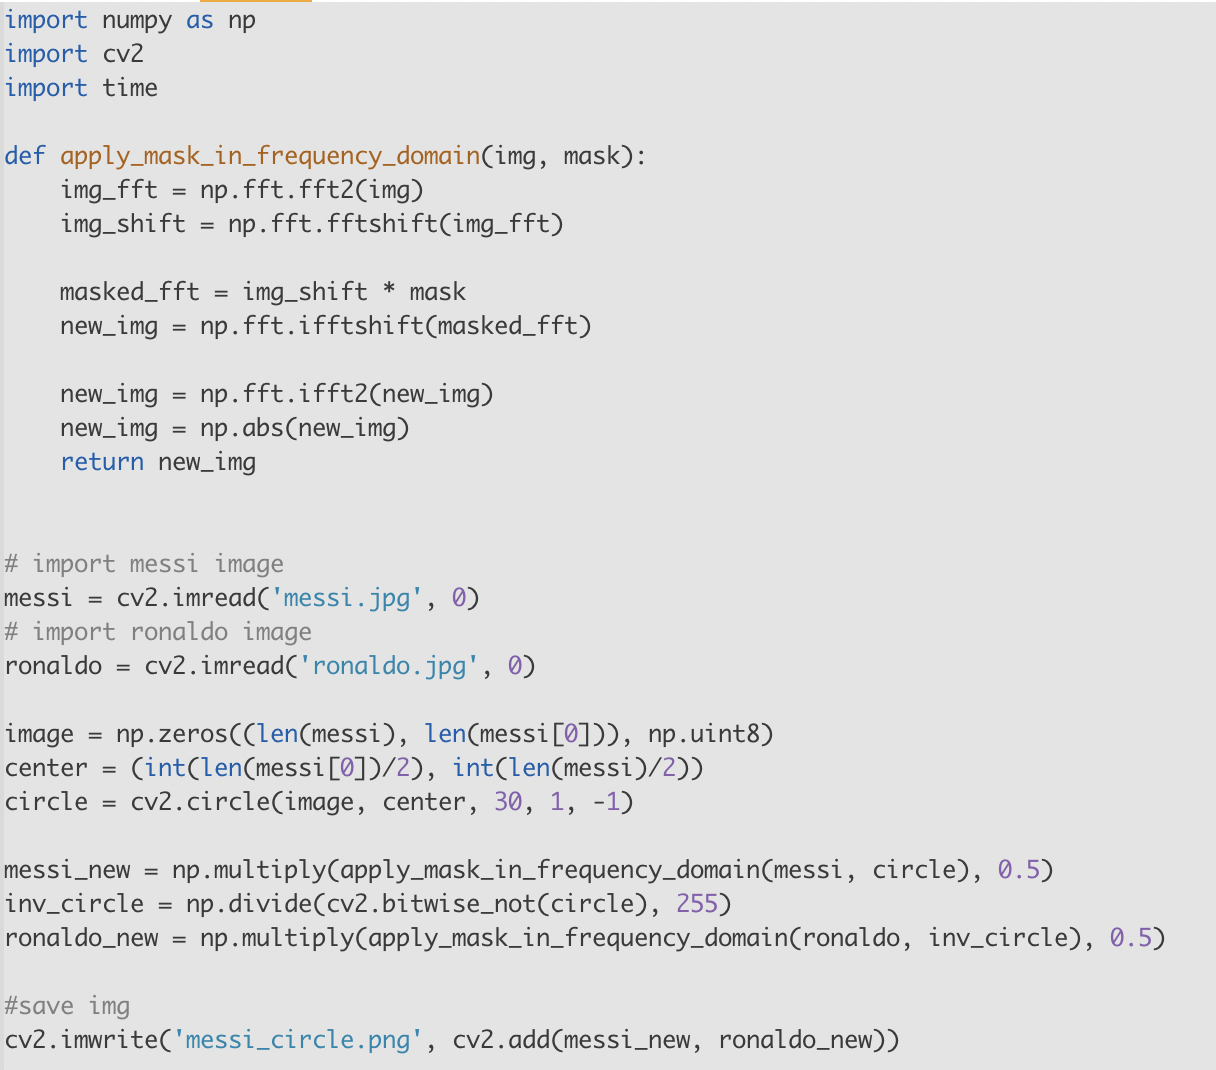
\includegraphics[width=\textwidth]{q2b.png}
    \caption{Hybrid Image Code}
\end{figure}

\subsection{Removing Noise}

\begin{figure}[H]
    \centering
    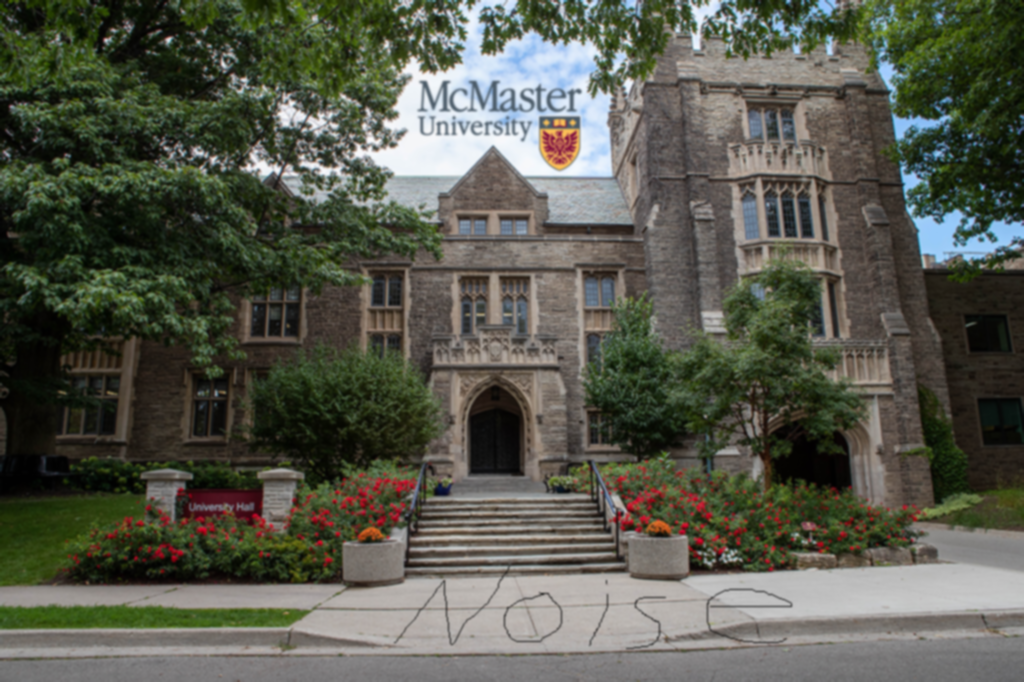
\includegraphics[width=\textwidth]{img3_gauss.png}
    \caption{Gaussian Blur}
\end{figure}
\begin{figure}[H]
    \centering
    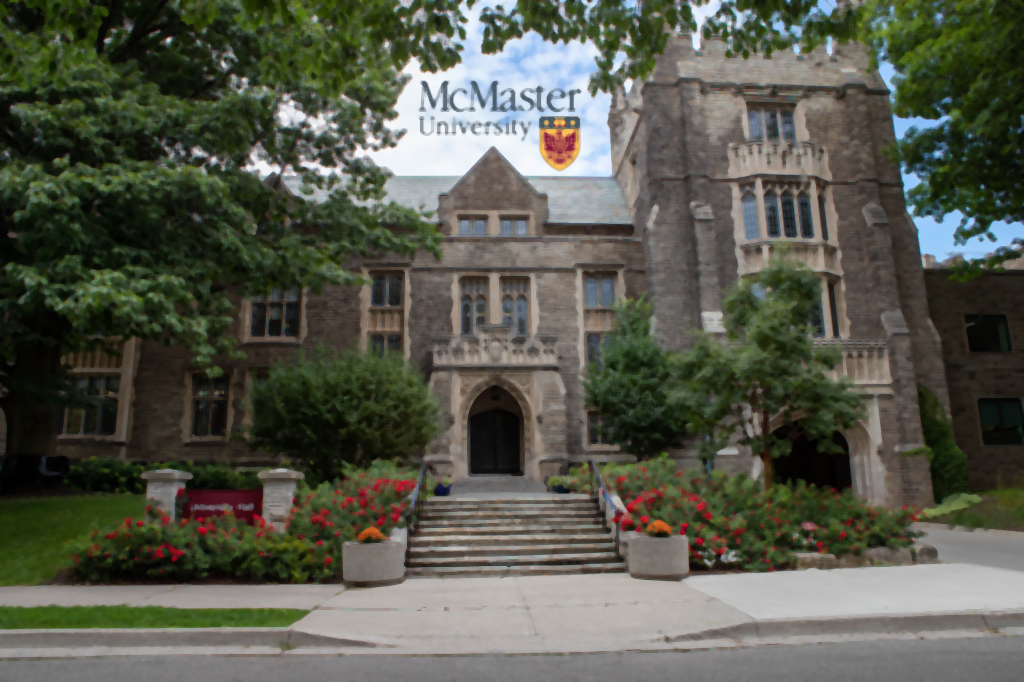
\includegraphics[width=\textwidth]{img3_median.png}
    \caption{Gaussian Blur}
\end{figure}

As we can clearly see, the median blur was far more effective at removing the noise from the image than the Gaussian blur. This is because the Gaussian blur acts as a sort of average, so big outliers still affect the final value, whereas with the median filter, a single big outlier will be discarded completely.


\begin{figure}[H]
    \centering
    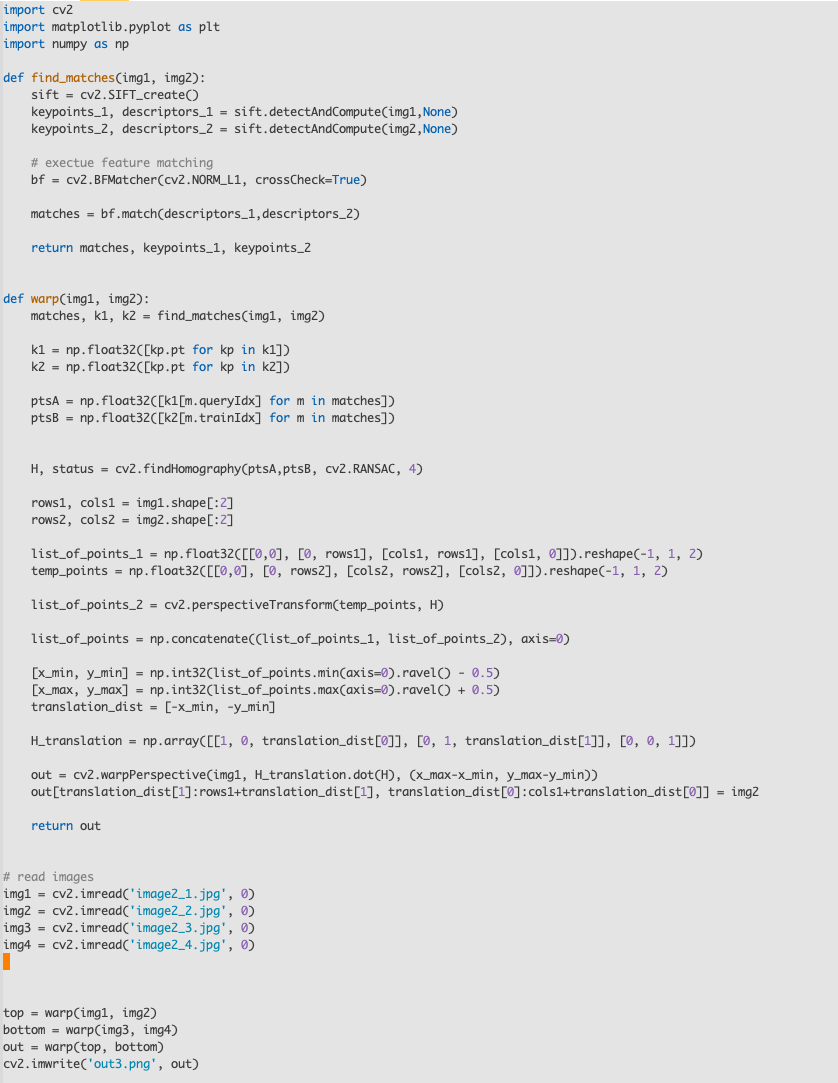
\includegraphics[width=\textwidth]{q3.png}
    \caption{Median and Gaussian Blur Code}
\end{figure}

\subsection{Histogram Equalization of Color Images}

\subsubsection{RGB Equalization}

\begin{figure}[H]
    \centering
    \subfloat[\centering Original Blue Channel Histogram]{{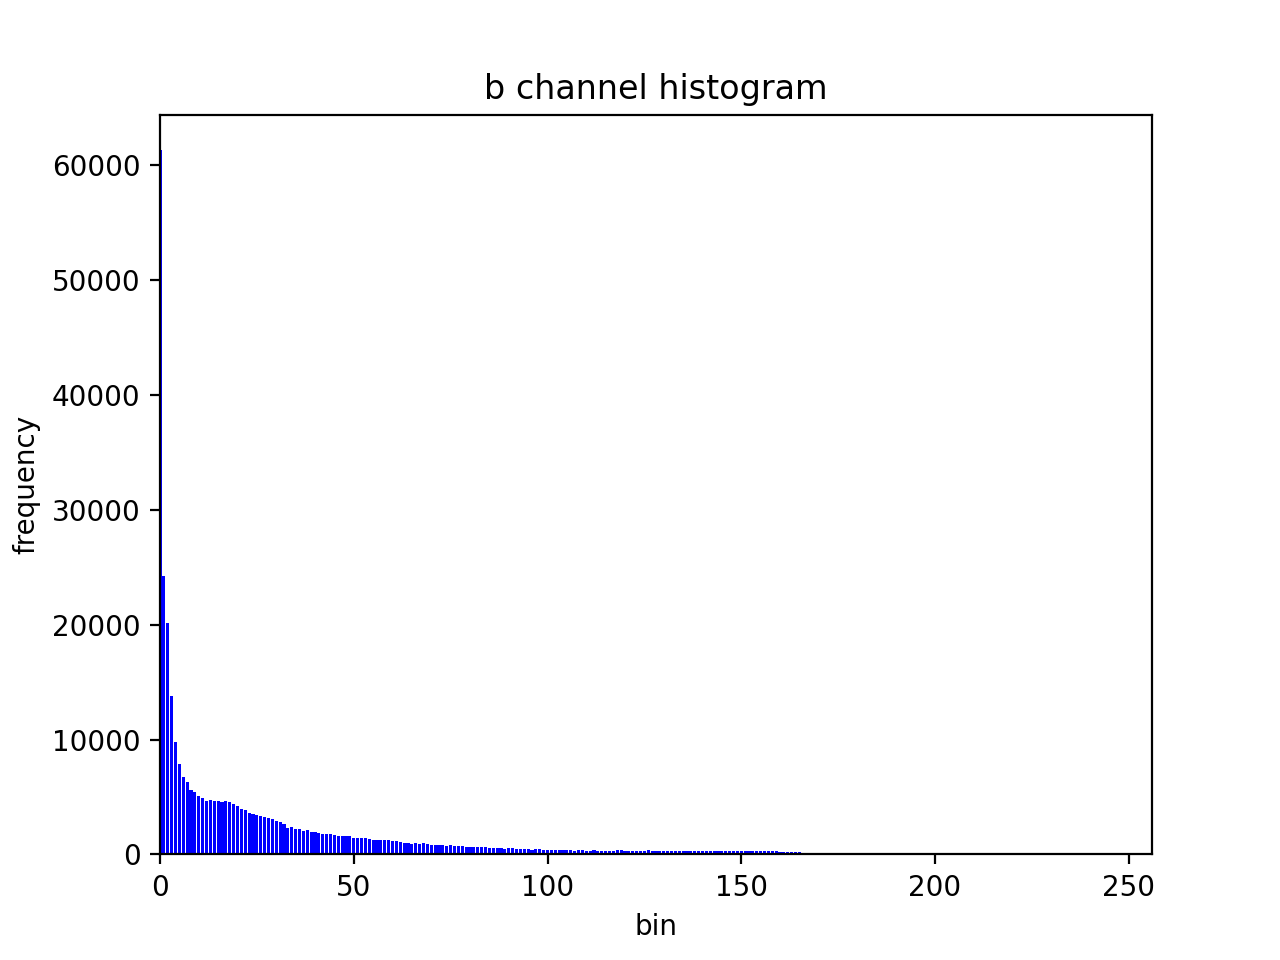
\includegraphics[width=.45\textwidth]{q4/b_hist_before.png} }}%
    \qquad
    \subfloat[\centering Equalized Blue Channel Histogram]{{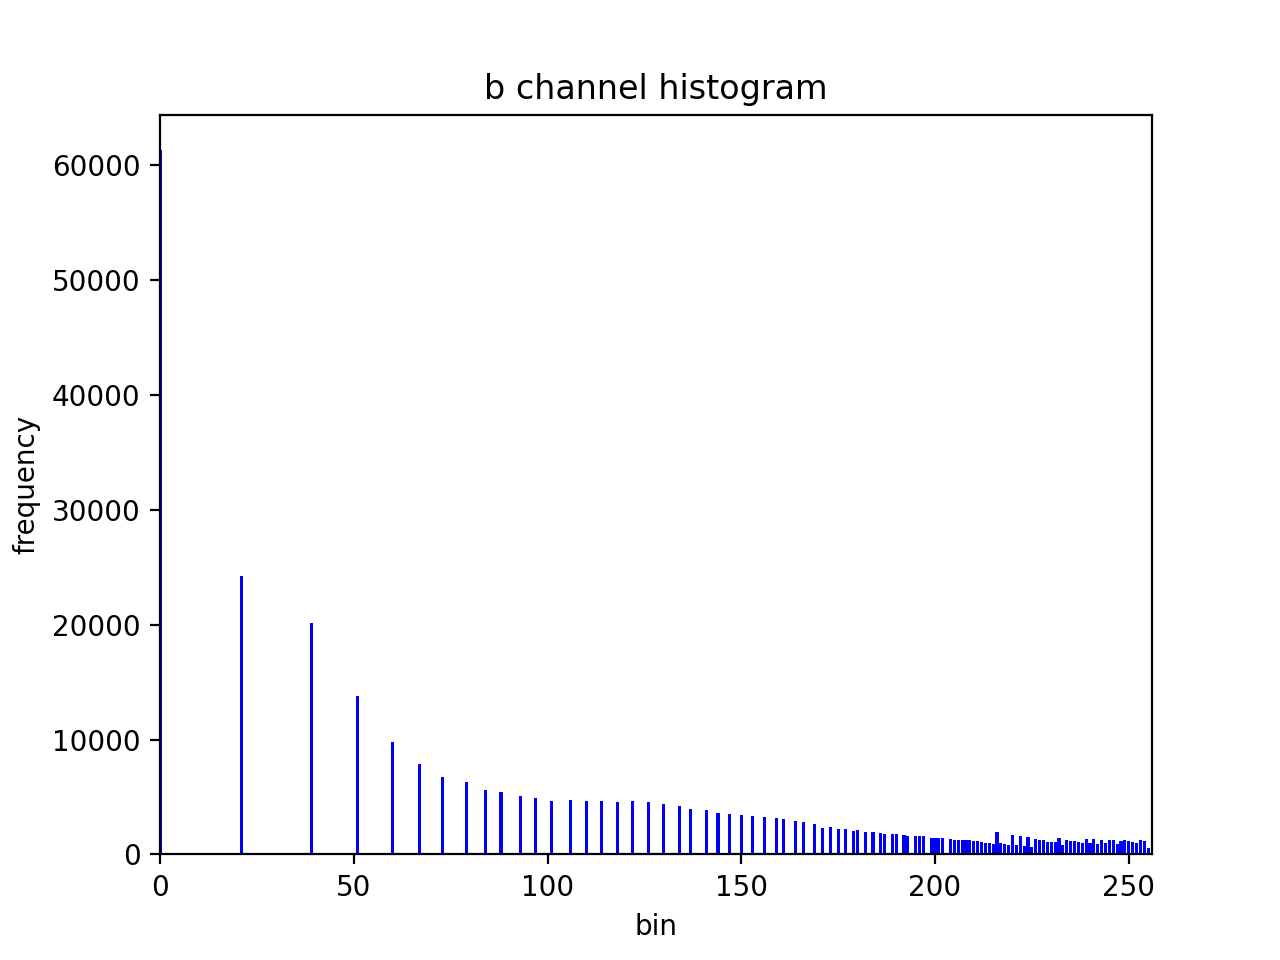
\includegraphics[width=.45\textwidth]{q4/b_hist_after.png} }}%
    \caption{Blue Channel Histogram Before and After Equalization}%
\end{figure}

\begin{figure}[H]
    \centering
    \subfloat[\centering Original Green Channel Histogram]{{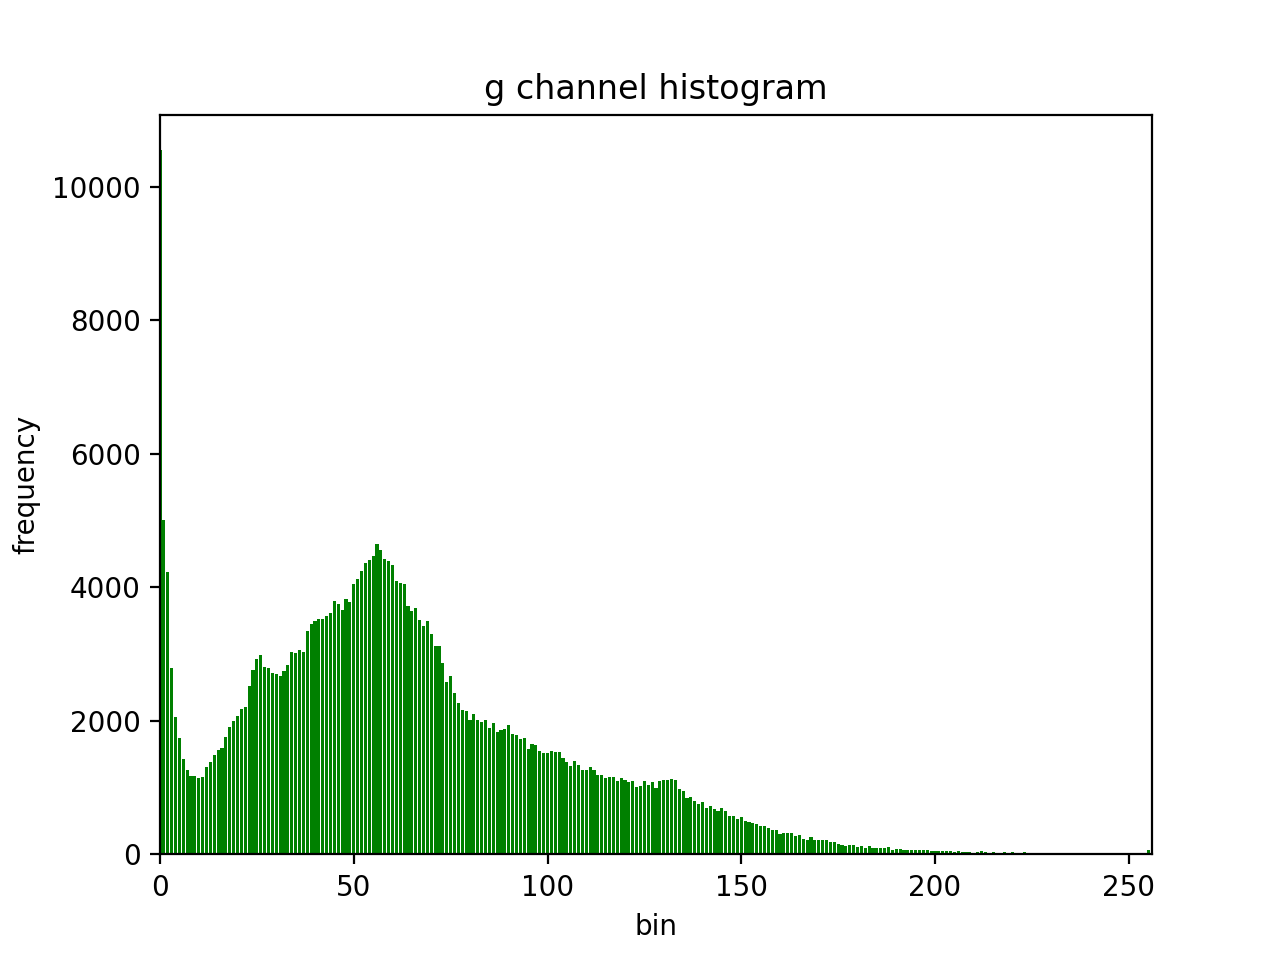
\includegraphics[width=.45\textwidth]{q4/g_hist_before.png} }}%
    \qquad
    \subfloat[\centering Equalized Green Channel Histogram]{{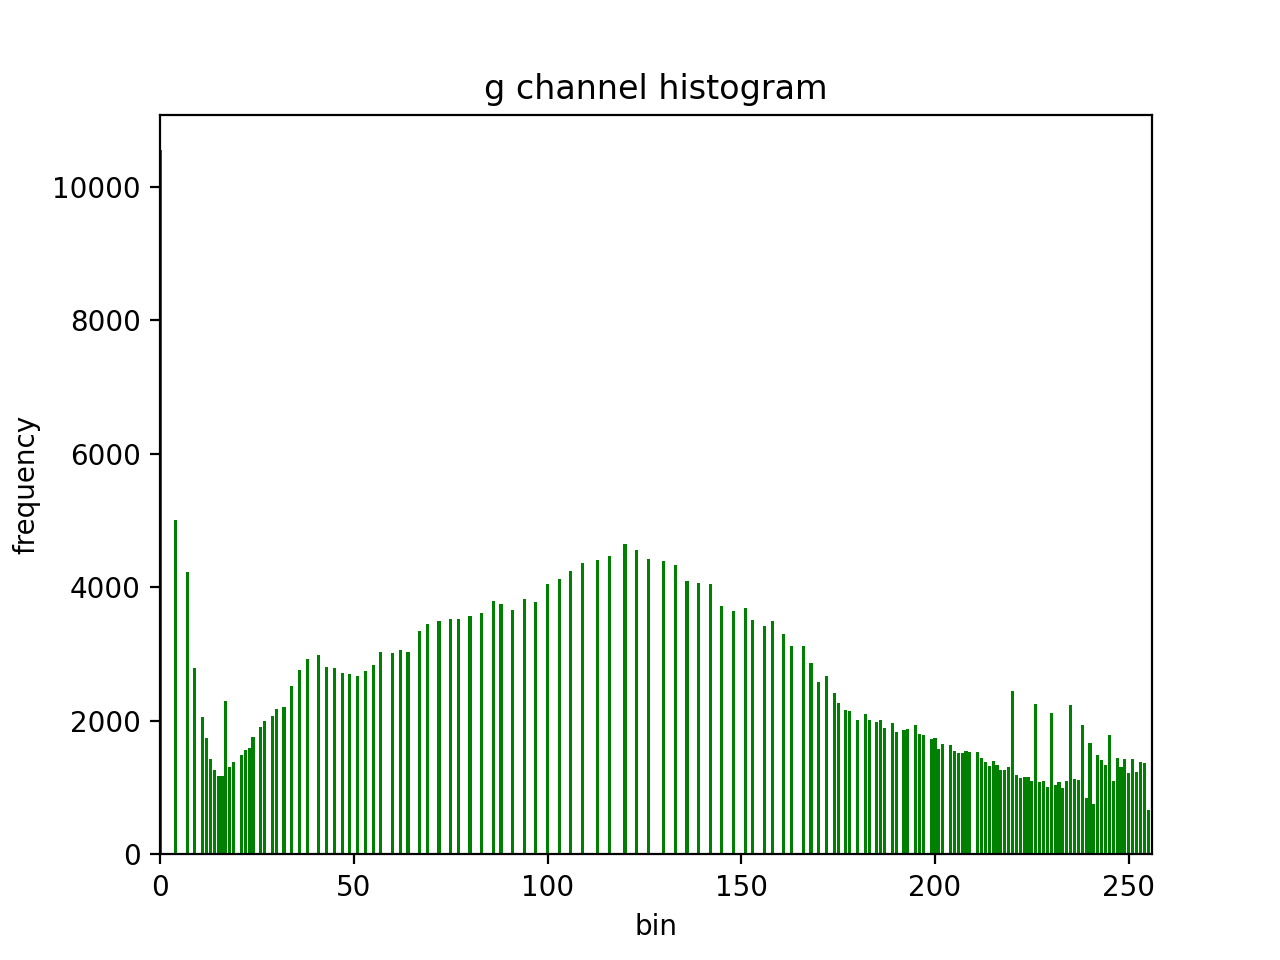
\includegraphics[width=.45\textwidth]{q4/g_hist_after.png} }}%
    \caption{Green Channel Histogram Before and After Equalization}%
\end{figure}

\begin{figure}[H]
    \centering
    \subfloat[\centering Original Red Channel Histogram]{{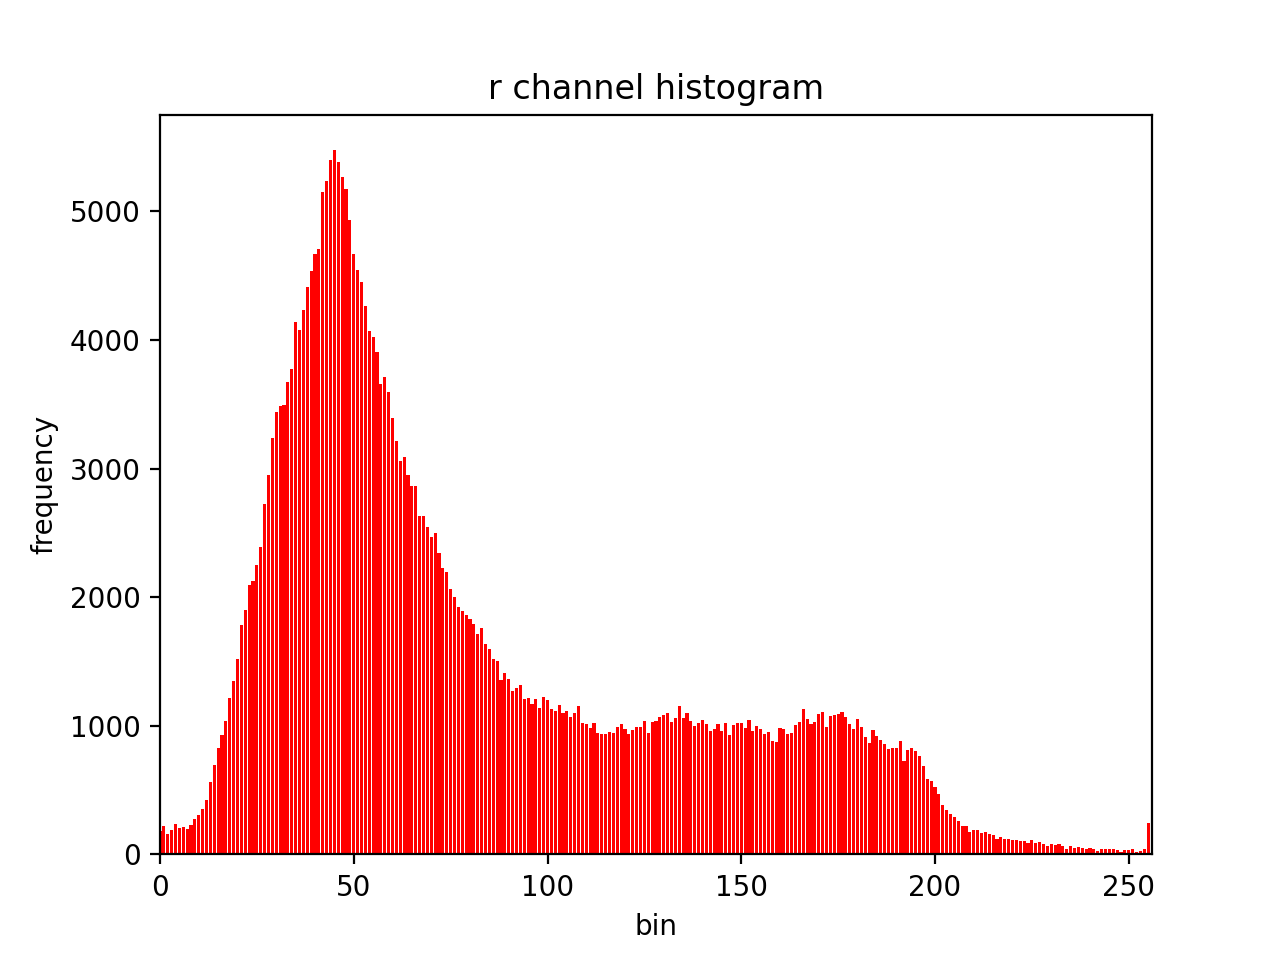
\includegraphics[width=.45\textwidth]{q4/r_hist_before.png} }}%
    \qquad
    \subfloat[\centering Equalized Red Channel Histogram]{{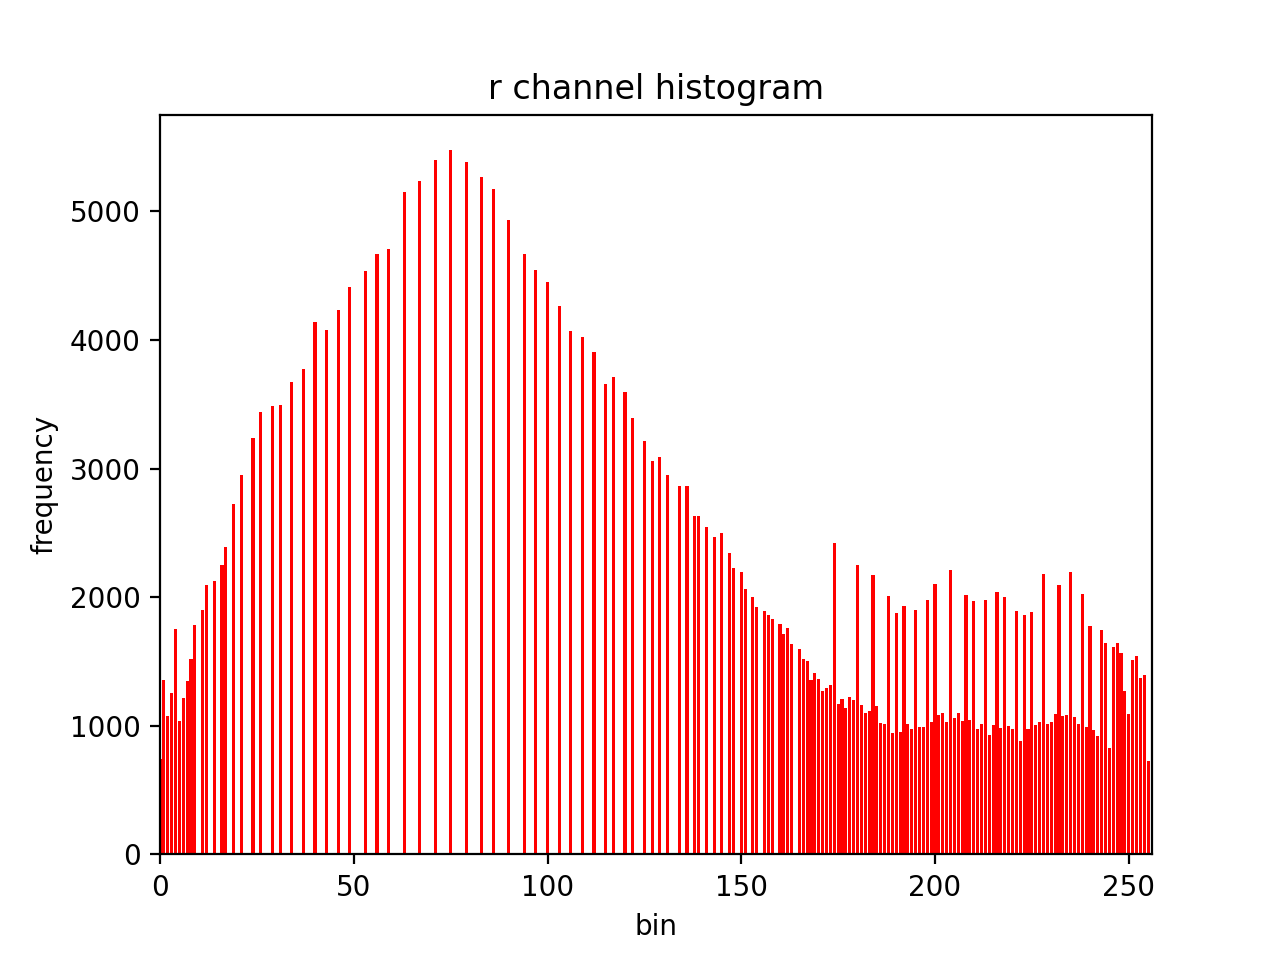
\includegraphics[width=.45\textwidth]{q4/r_hist_after.png} }}%
    \caption{Red Channel Histogram Before and After Equalization}%
\end{figure}

\begin{figure}[H]
    \centering
    \subfloat[\centering Original Image]{{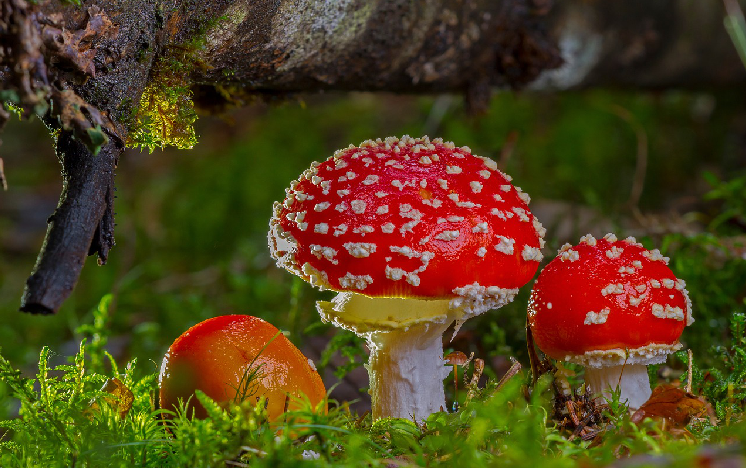
\includegraphics[width=.45\textwidth]{q4/img4.png} }}%
    \qquad
    \subfloat[\centering Equalized Image]{{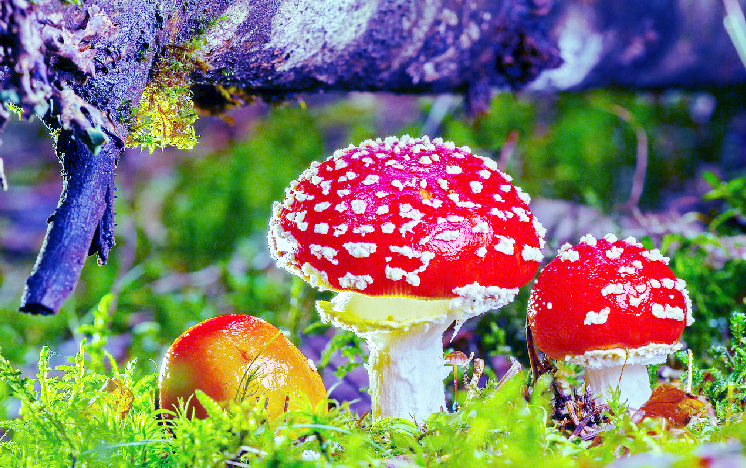
\includegraphics[width=.45\textwidth]{q4/img4_rgb_he.png} }}%
    \caption{Image Before and After RGB Equalization}%
\end{figure}

\subsection{Histogram Equalization of Color Images}

\subsubsection{LAB Equalization}

\begin{figure}[H]
    \centering
    \subfloat[\centering Original L Channel Histogram]{{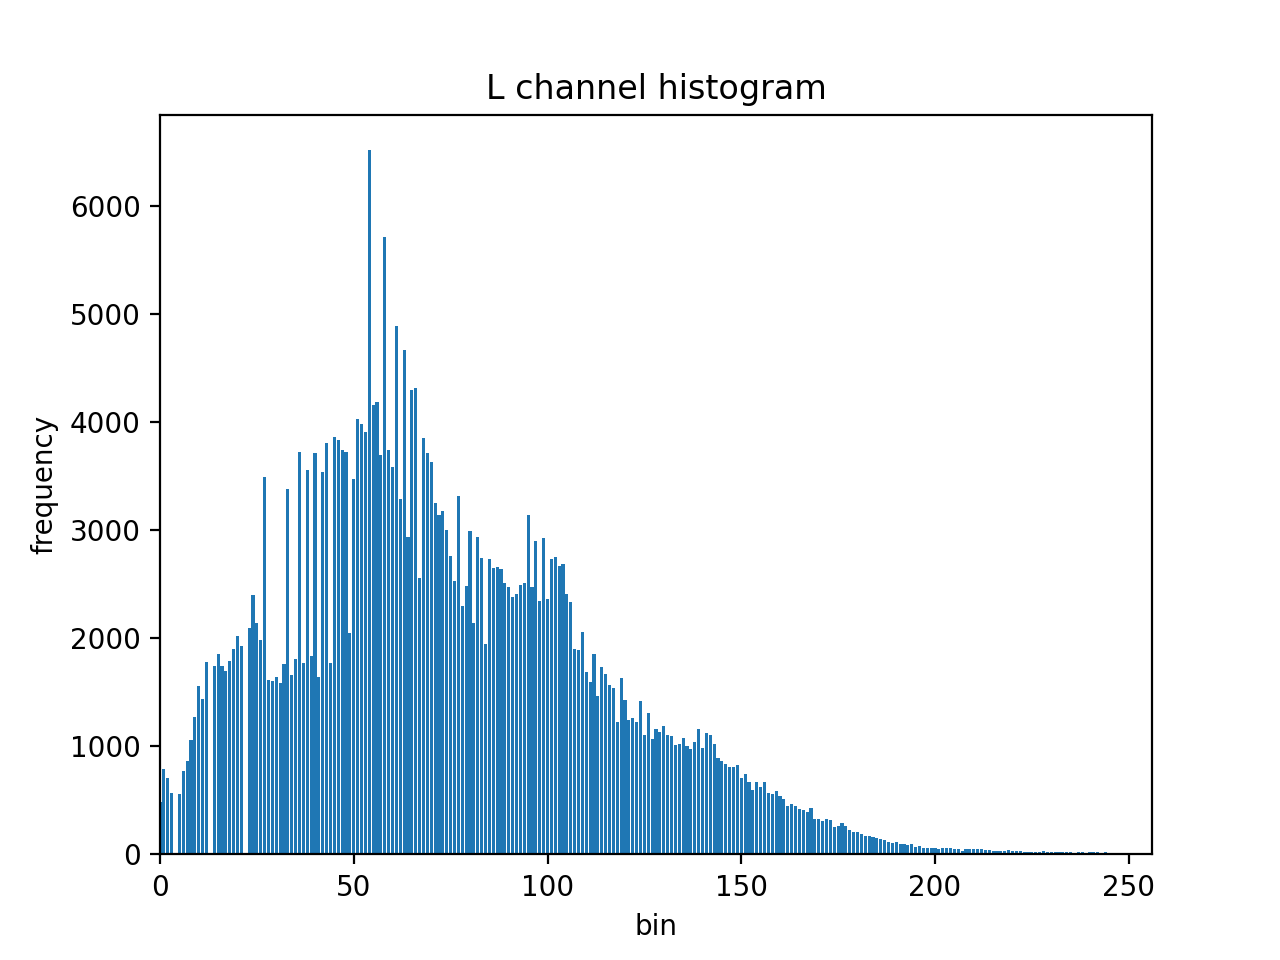
\includegraphics[width=.45\textwidth]{q4/l_hist_before.png} }}%
    \qquad
    \subfloat[\centering Equalized L Channel Histogram]{{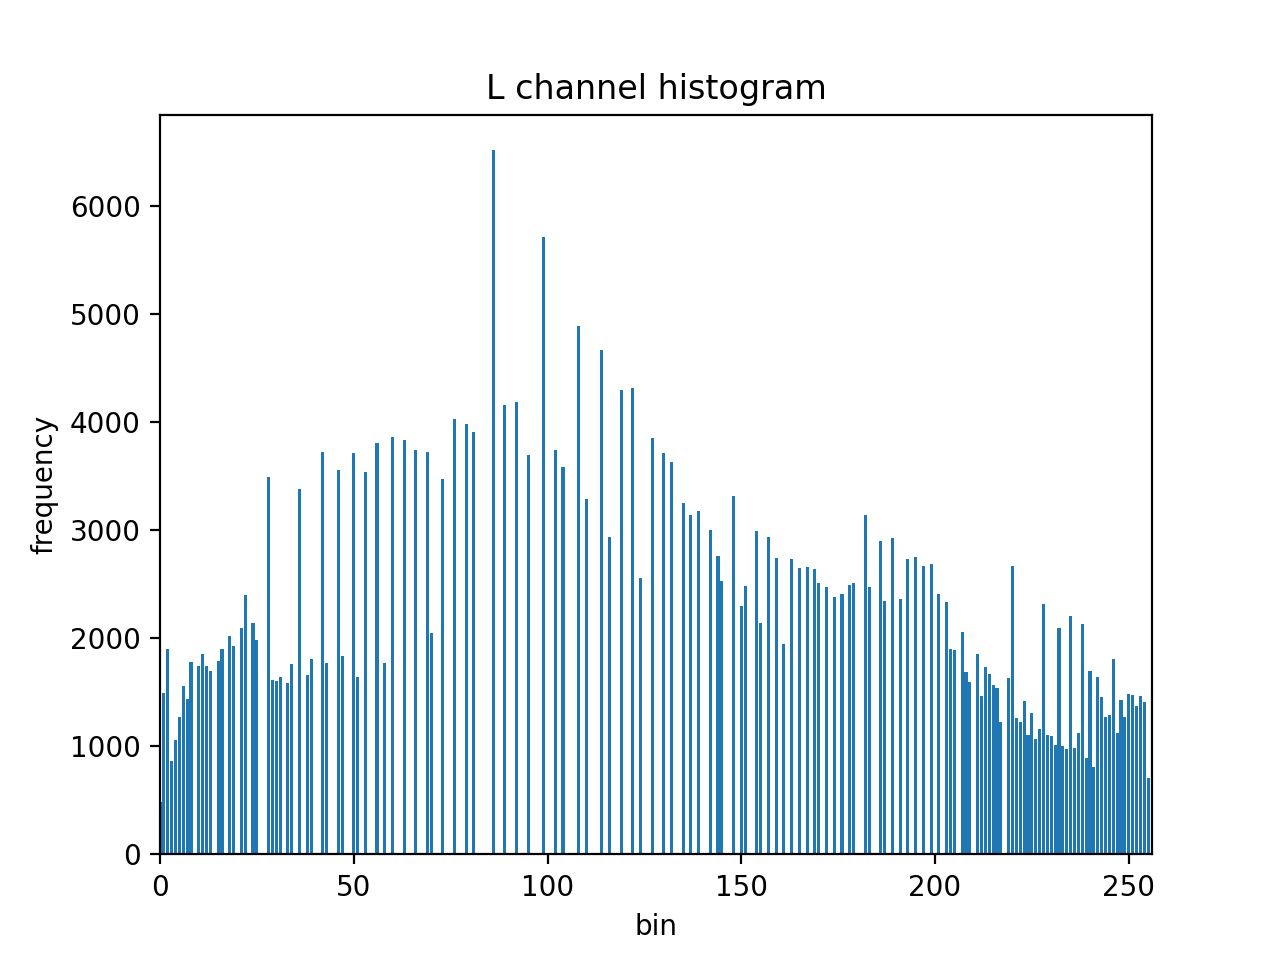
\includegraphics[width=.45\textwidth]{q4/l_hist_after.png} }}%
    \caption{L Channel Histogram Before and After Equalization}%
\end{figure}

\begin{figure}[H]
    \centering
    \subfloat[\centering Original Image]{{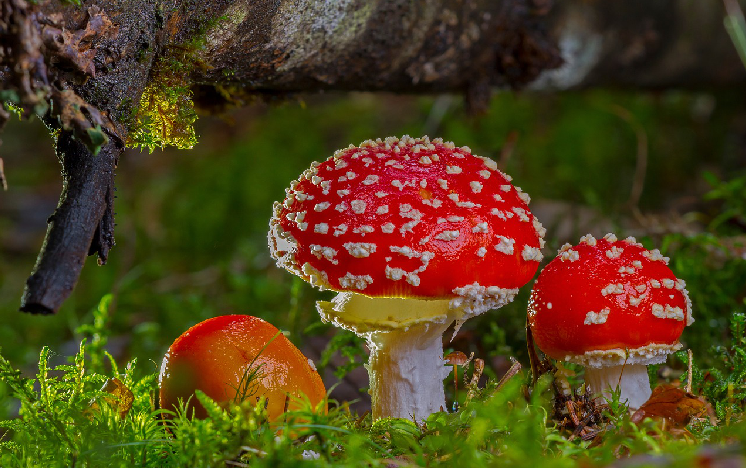
\includegraphics[width=.45\textwidth]{q4/img4.png} }}%
    \qquad
    \subfloat[\centering Equalized Image]{{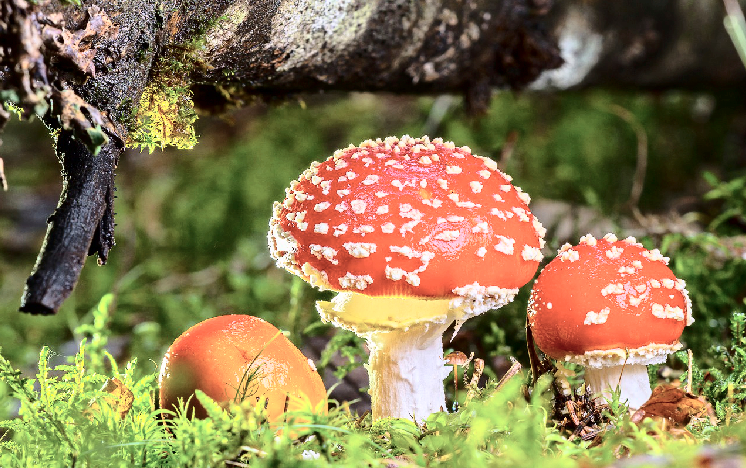
\includegraphics[width=.45\textwidth]{q4/img4_lab_he.png} }}%
    \caption{Image Before and After LAB Equalization}%
\end{figure}

\subsubsection{RGB Equalization with CLAHE}

\begin{figure}[H]
    \centering
    \subfloat[\centering Original Blue Channel Histogram]{{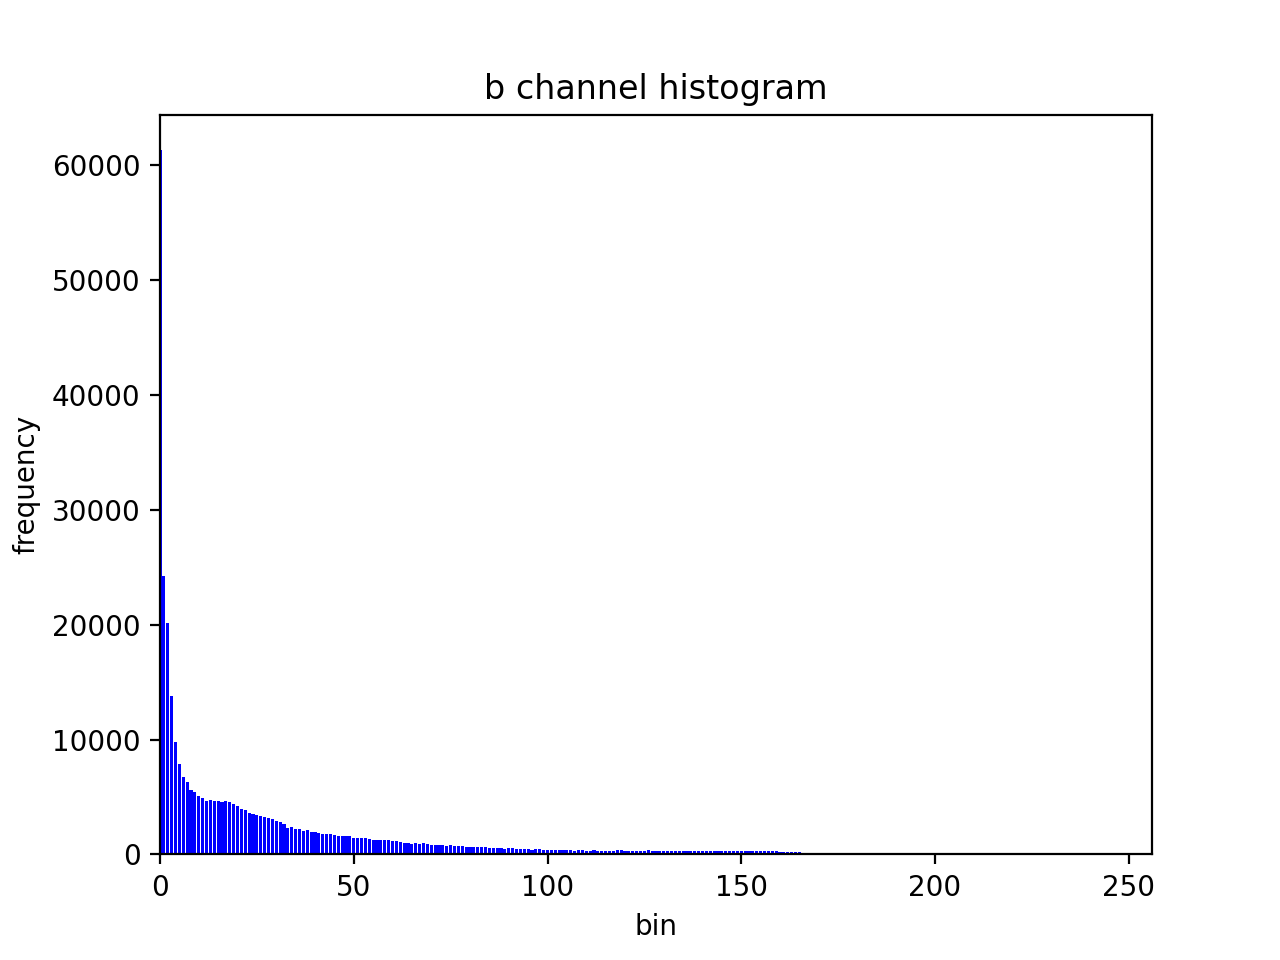
\includegraphics[width=.45\textwidth]{q4/b_hist_before.png} }}%
    \qquad
    \subfloat[\centering Equalized Blue Channel Histogram]{{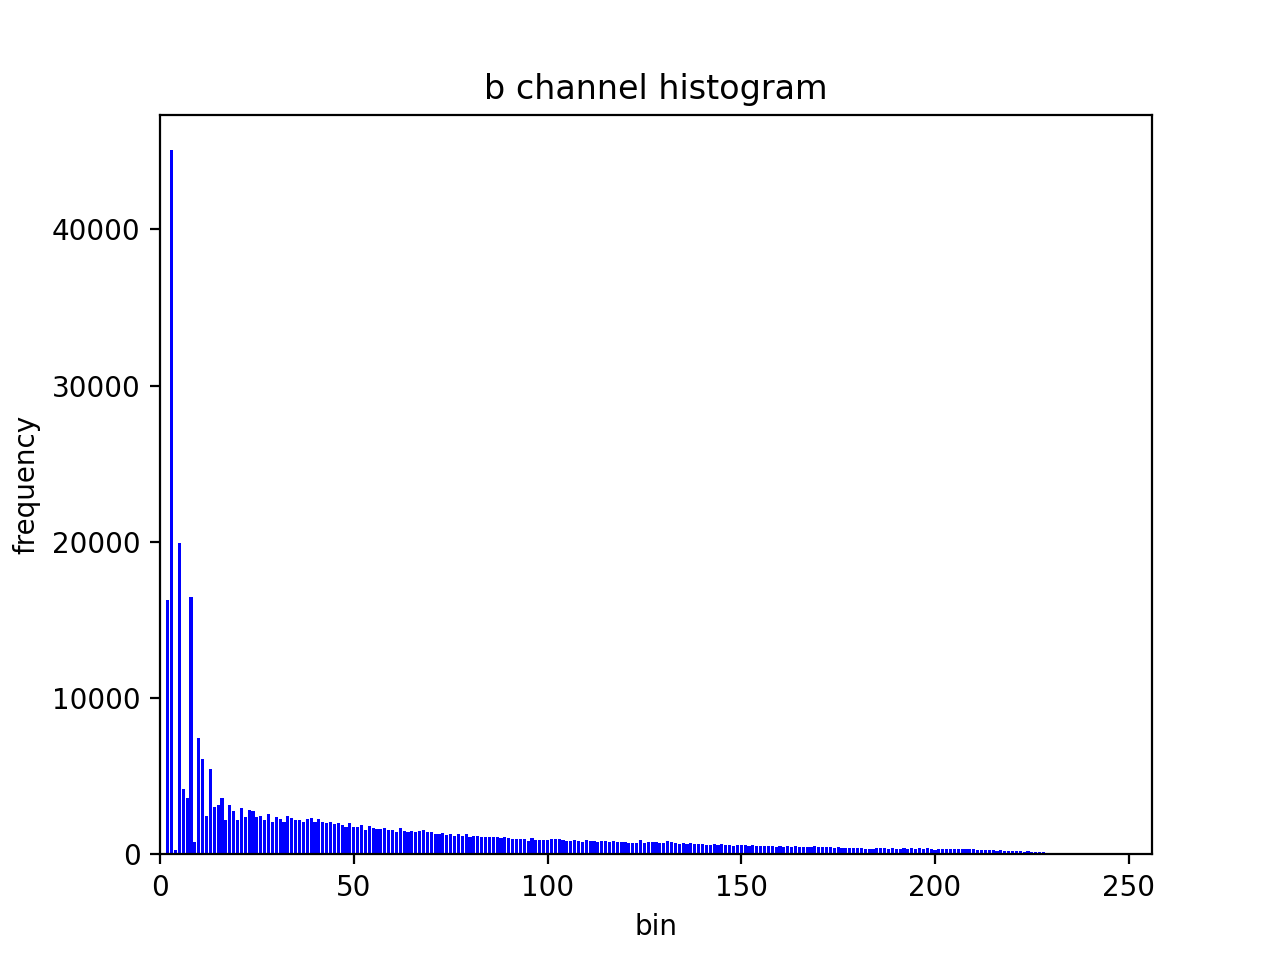
\includegraphics[width=.45\textwidth]{q4/b_hist_after_clahe.png} }}%
    \caption{Blue Channel Histogram Before and After CLAHE Equalization}%
\end{figure}

\begin{figure}[H]
    \centering
    \subfloat[\centering Original Green Channel Histogram]{{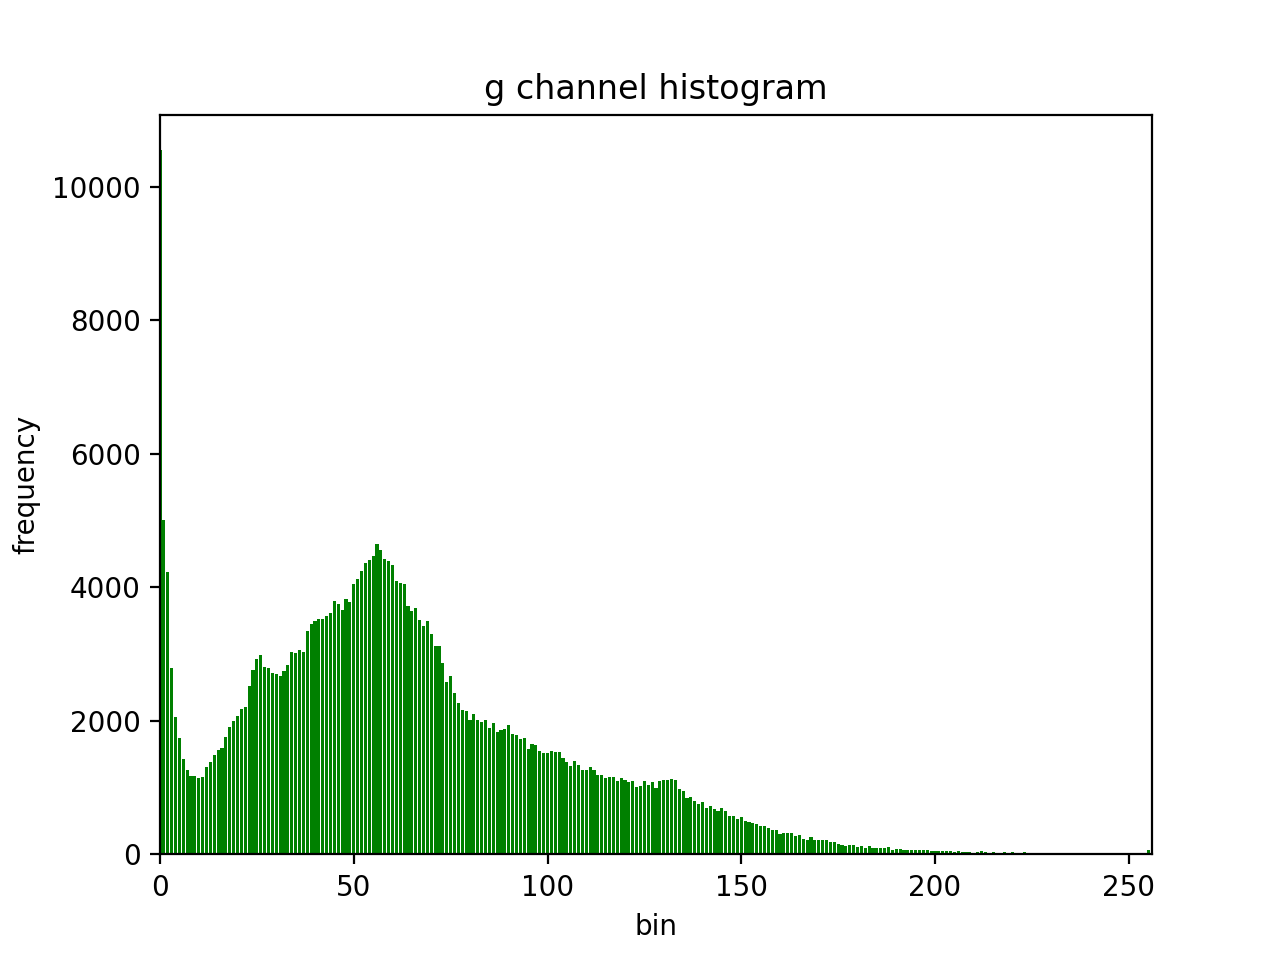
\includegraphics[width=.45\textwidth]{q4/g_hist_before.png} }}%
    \qquad
    \subfloat[\centering Equalized Green Channel Histogram]{{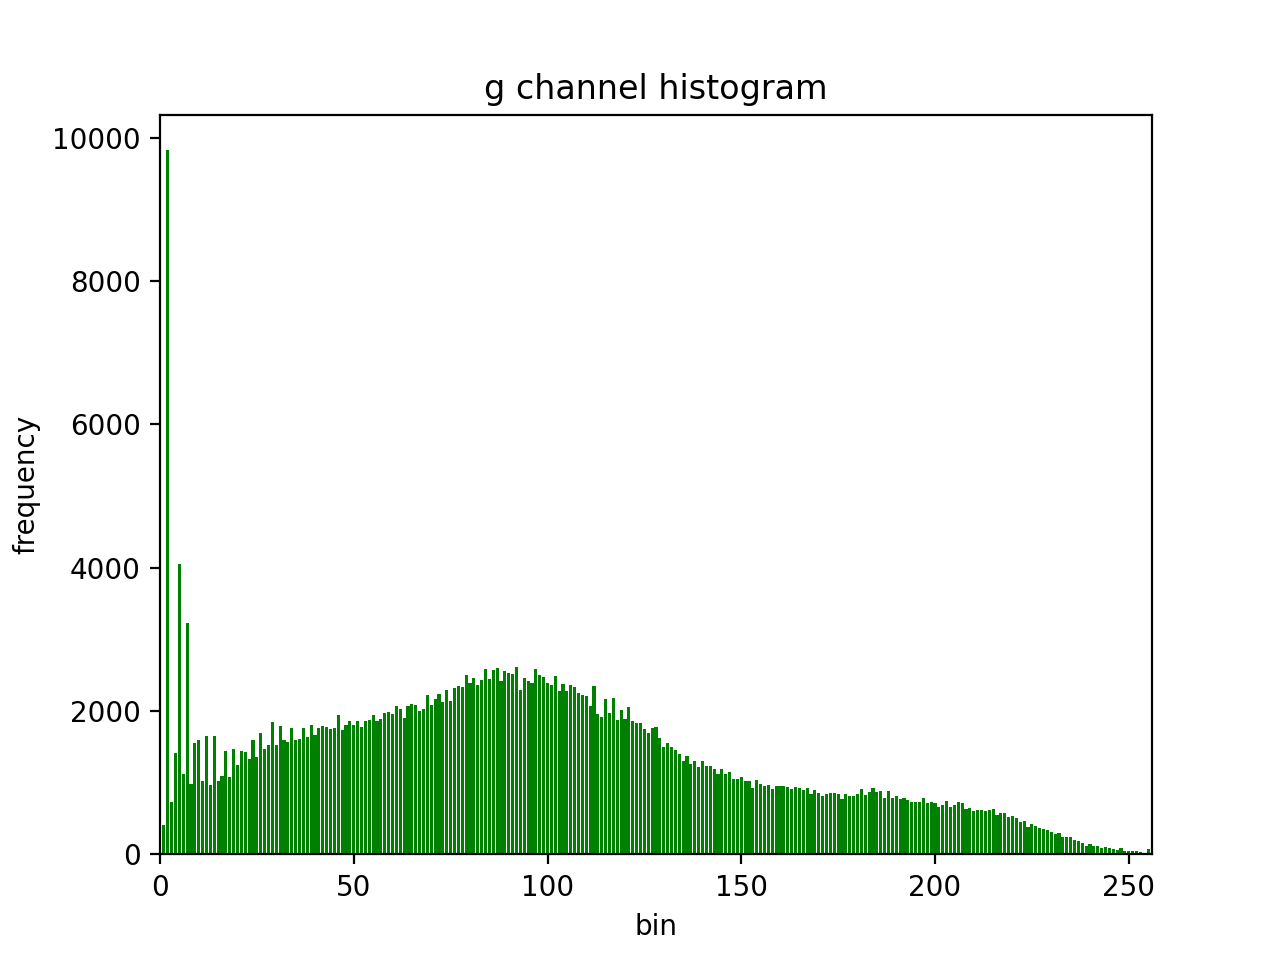
\includegraphics[width=.45\textwidth]{q4/g_hist_after_clahe.png} }}%
    \caption{Green Channel Histogram Before and After CLAHE Equalization}%
\end{figure}

\begin{figure}[H]
    \centering
    \subfloat[\centering Original Red Channel Histogram]{{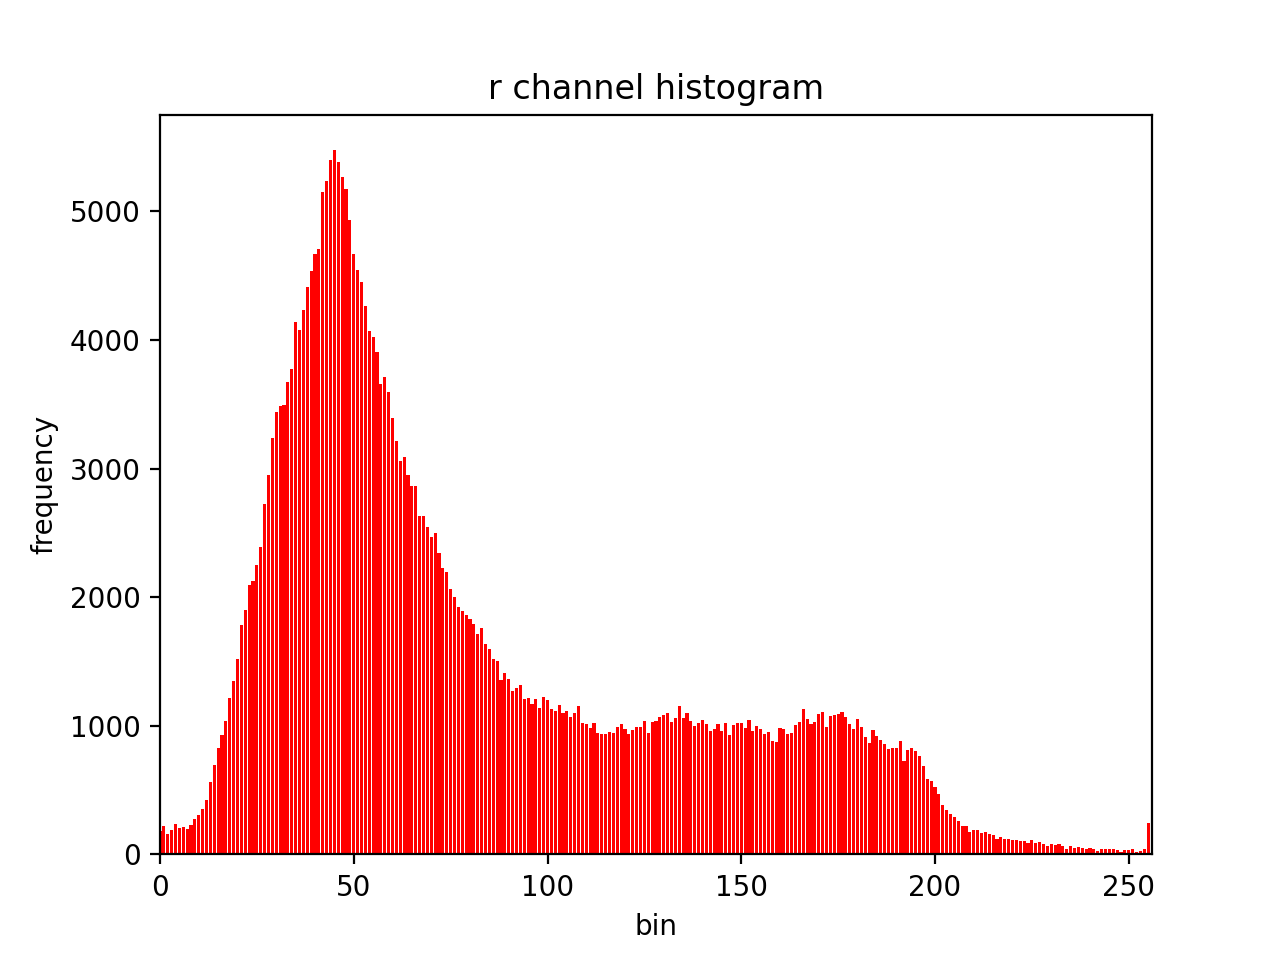
\includegraphics[width=.45\textwidth]{q4/r_hist_before.png} }}%
    \qquad
    \subfloat[\centering Equalized Red Channel Histogram]{{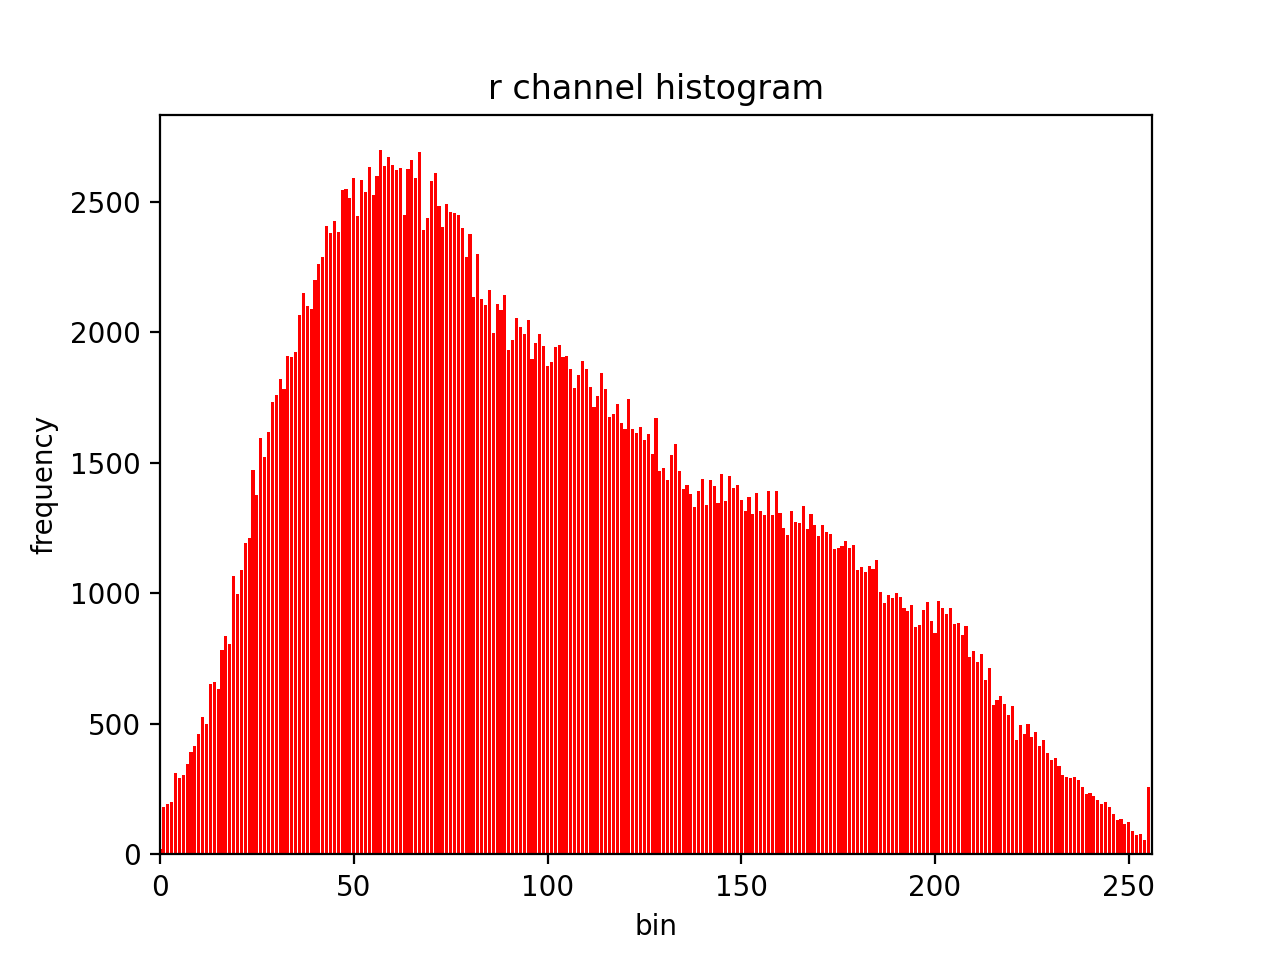
\includegraphics[width=.45\textwidth]{q4/r_hist_after_clahe.png} }}%
    \caption{Red Channel Histogram Before and After CLAHE Equalization}%
\end{figure}

\begin{figure}[H]
    \centering
    \subfloat[\centering Original Image]{{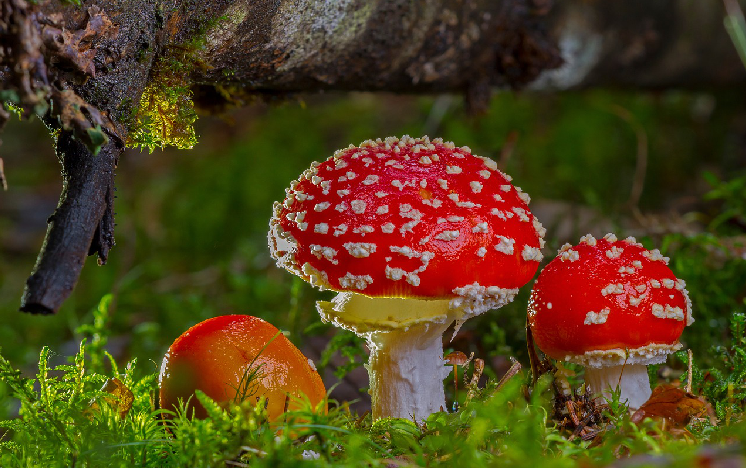
\includegraphics[width=.45\textwidth]{q4/img4.png} }}%
    \qquad
    \subfloat[\centering Equalized Image]{{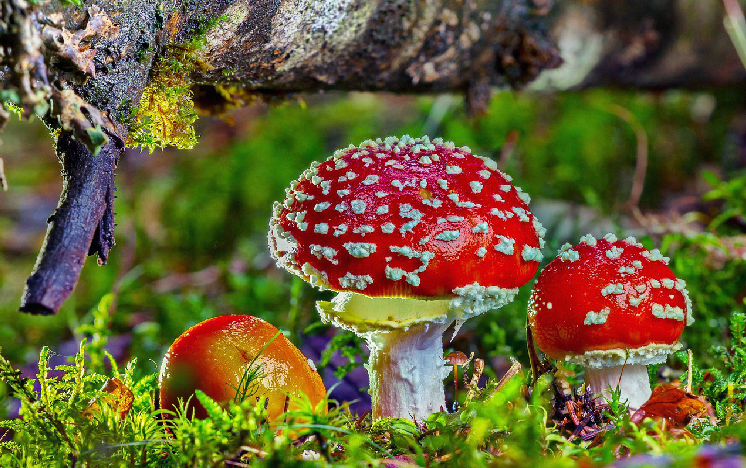
\includegraphics[width=.45\textwidth]{q4/img4_rgb_heCLAHE.png} }}%
    \caption{Image Before and After CLAHE RGB Equalization}%
\end{figure}

\subsection{Histogram Equalization of Color Images}

\subsubsection{LAB Equalization with CLAHE}

\begin{figure}[H]
    \centering
    \subfloat[\centering Original L Channel Histogram]{{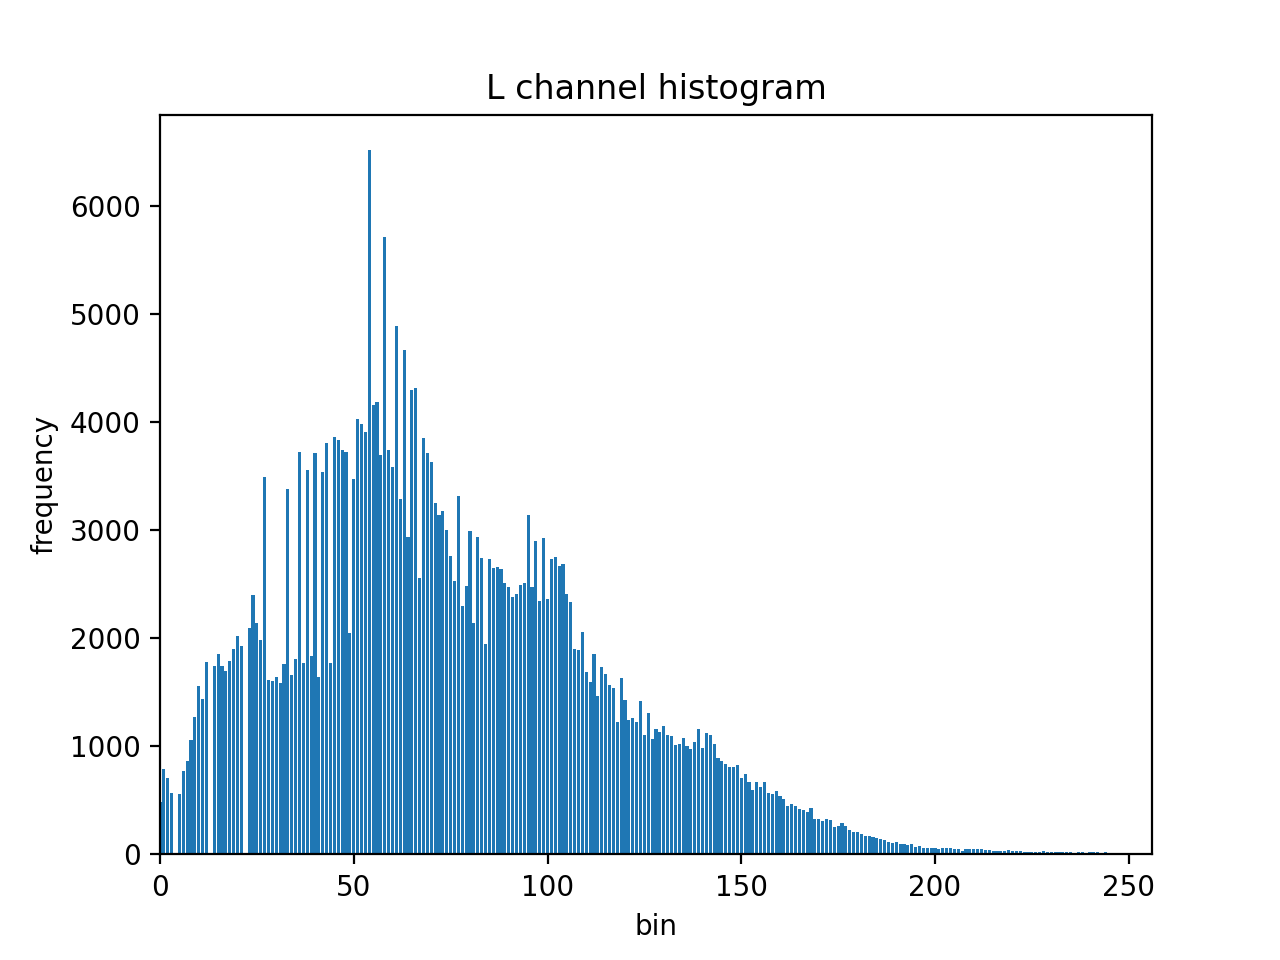
\includegraphics[width=.45\textwidth]{q4/l_hist_before.png} }}%
    \qquad
    \subfloat[\centering Equalized L Channel Histogram]{{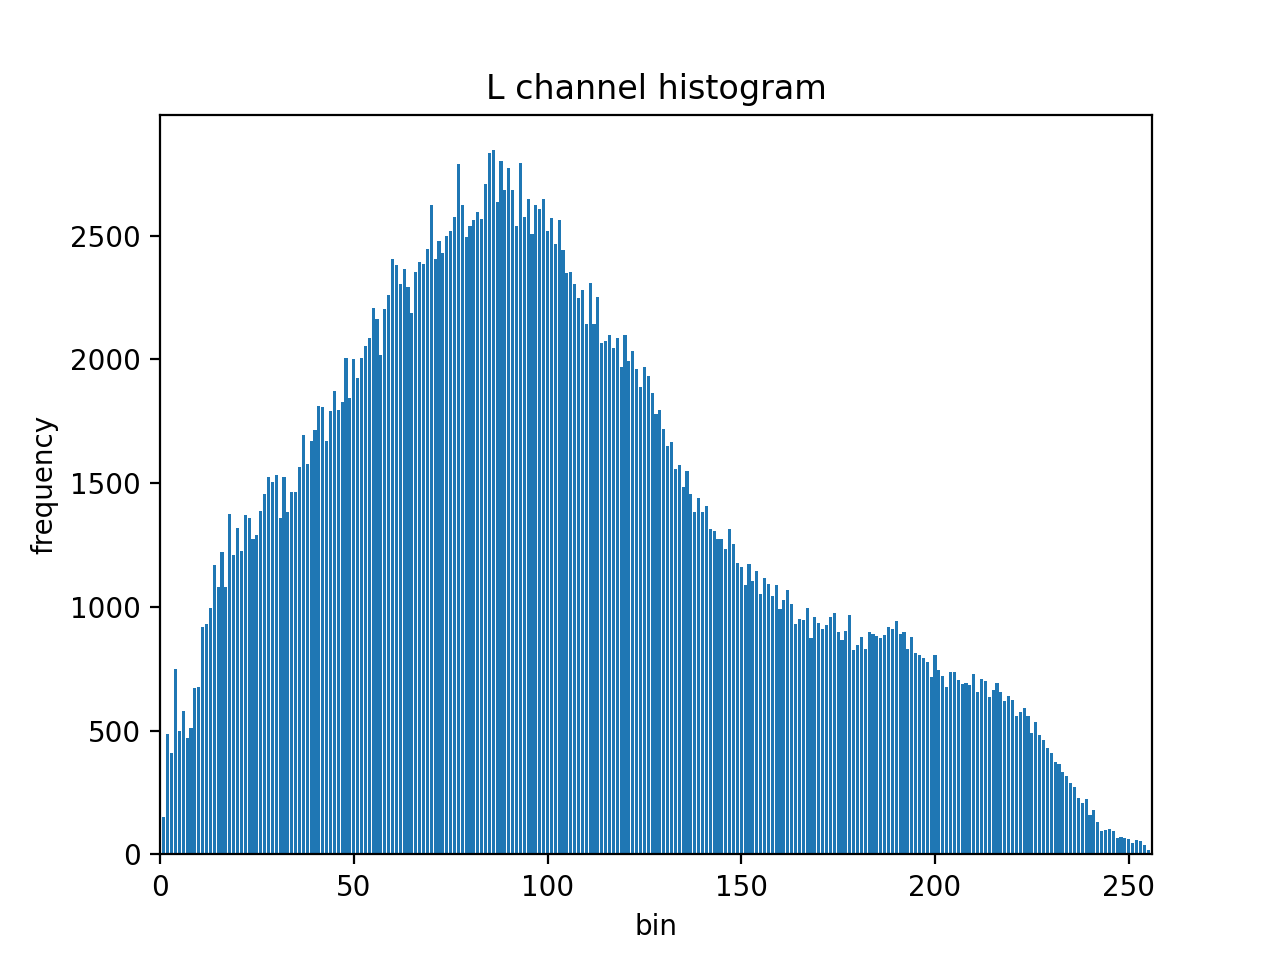
\includegraphics[width=.45\textwidth]{q4/l_hist_after_clahe.png} }}%
    \caption{L Channel Histogram Before and After CLAHE Equalization}%
\end{figure}

\begin{figure}[H]
    \centering
    \subfloat[\centering Original Image]{{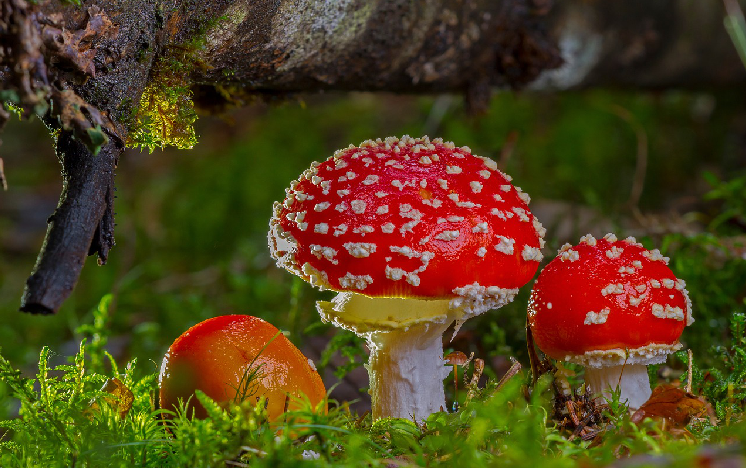
\includegraphics[width=.45\textwidth]{q4/img4.png} }}%
    \qquad
    \subfloat[\centering Equalized Image]{{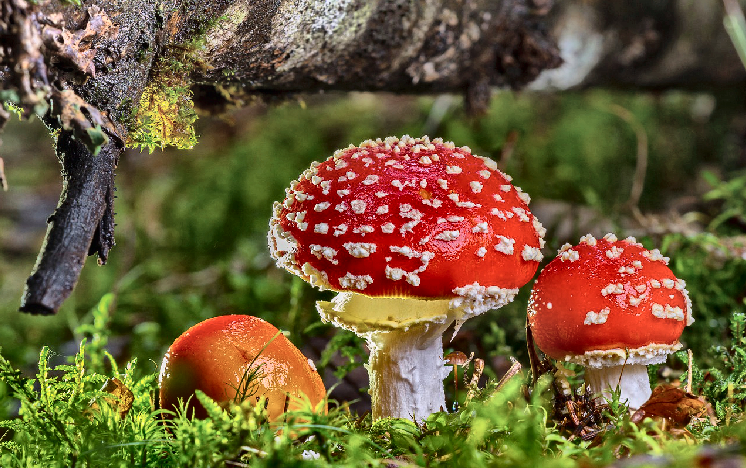
\includegraphics[width=.45\textwidth]{q4/img4_lab_heCLAHE.png} }}%
    \caption{Image Before and After CLAHE LAB Equalization}%
\end{figure}

\subsubsection{Analysis}

We can rank the effectiveness of the equalization from best to worst in the following order:
\begin{enumerate}
  \item LAB with CLAHE
  \item LAB (global)
  \item RGB with CLAHE
  \item RGB (global)
\end{enumerate}

Both techniques that involve equalizing the RGB channels independently, produce bad results because we are simply equalizing each channel with no regard for the other channels, resulting in the colors changing instead of only the contrast. This is evident in Figures 17 and 23, where we see the saturation of the colors greatly increase.

The LAB color space contains color information in the $A$ and $B$ channels, while the $L$ channel contains only \textit{lightness} information. Therefore, by equalizing the $L$ channel, we can improve the contrast in the image without changing the color information as evident in Figures 19 and 25. 

\subsubsection{Code}

\begin{figure}[H]
    \centering
    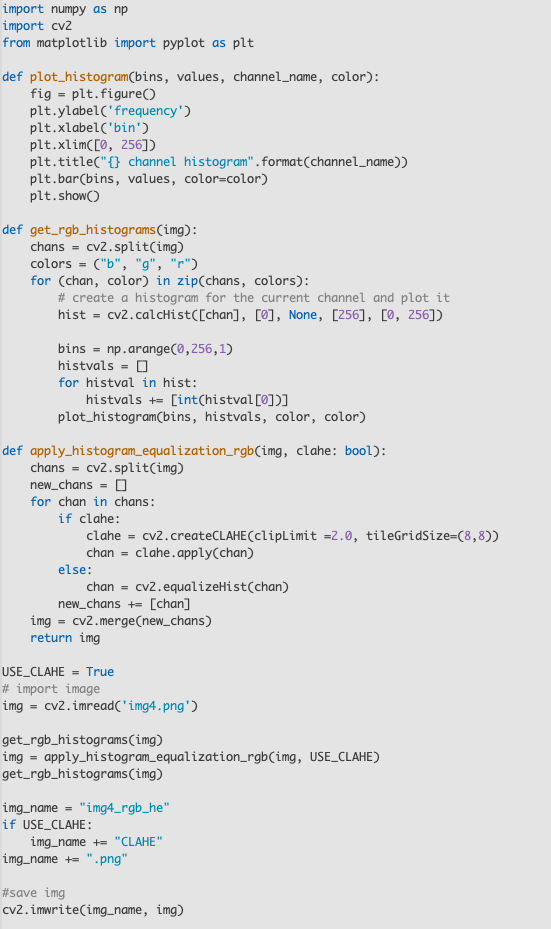
\includegraphics[width=.9\textwidth]{q4/q4-rgb.png}
    \caption{RGB Equalization Code}
\end{figure}

\begin{figure}[H]
    \centering
    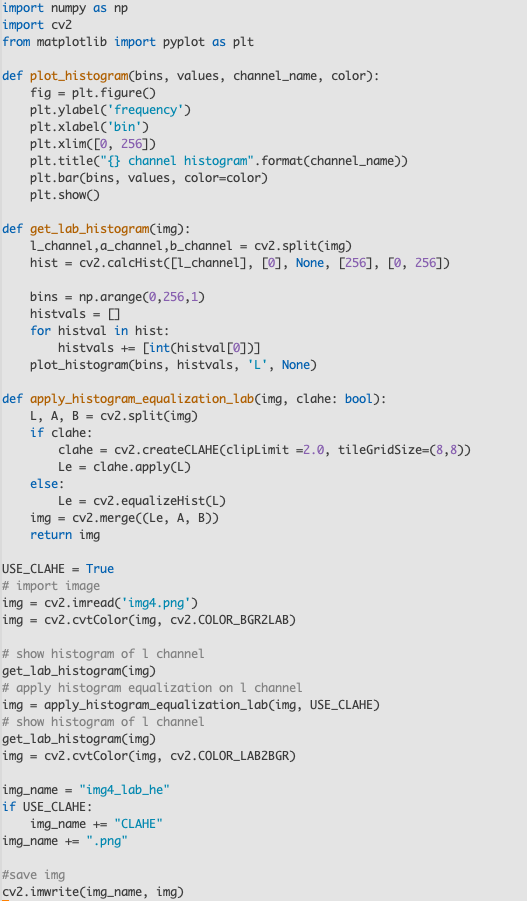
\includegraphics[width=.9\textwidth]{q4/q4-lab.png}
    \caption{LAB Equalization Code}
\end{figure}

\end{document}
